\documentclass[aps,prb,twocolumn,superscriptaddress,amsmath,amssymb,floatfix]{revtex4}
%\documentclass[aps,prb,onecolumn,preprint,superscriptaddress,amsmath,amssymb,floatfix]{revtex4}
%\documentclass[aps,prl,onecolumn,groupedaddress,amsmath,amssymb,12pt]{revtex4}
\usepackage{graphicx}
\usepackage{ifthen}
\usepackage{dcolumn}% Align table columns on decimal point
\usepackage{bm}% bold math
\usepackage{multirow}
\usepackage{booktabs}
\usepackage{amsbsy}
\usepackage{amsmath}
\usepackage{amssymb}
\usepackage{subfigure}


%Definition of new commands
\newcommand{\f}[2]{\ensuremath{\frac{\displaystyle{#1}}{\displaystyle{#2}}}}
\newcommand{\lr}[1]{\langle{#1}\rangle}
\newcommand{\colv}[2] {\left(\begin{array}{c} #1 \\ #2 \end{array}\right)}
\renewcommand{\thefootnote}{\fnsymbol{footnote}}
\newcommand{\be} {\begin{eqnarray}}
\newcommand{\ee} {\end{eqnarray}}
%--------------------------------------------------------------------------
%EQ COMMANDS
%--------------------------------------------------------------------------
\newcommand{\two}{\mspace{-2.0mu}}
\newcommand{\four}{\mspace{-4.0mu}}
\newcommand{\plus}{\mspace{-4.5mu}+\mspace{-3.5mu}}
\newcommand{\minus}{\mspace{-4.5mu}-\mspace{-3.5mu}}
\newcommand{\pp}{'\mspace{-2.0mu}'}
\newcommand{\xlb}[4]{#1\ifthenelse{\equal{#2}{0}}{}{_{\alpha #2}}
\mspace{-2.0mu}\genfrac{(}{)}{0pt}{1}{\ifthenelse{\equal{#3}{0}}{0}{l #3}} 
{\ifthenelse{\equal{#4}{0}}{0}{b #4}}}

\newcommand{\xkv}[4]{#1\mspace{-5.0mu}\left(\mspace{-8.0mu}
\begin{smallmatrix}#2\four{}\four{}\mspace{-8.0mu}&\pmb{\kappa}#3\\&\nu 
#4\end{smallmatrix}\mspace{-5.0mu}\right)}

\newcommand{\evect}[6]{#1\mspace{-4.0mu}\left(\mspace{-8.0mu}
\begin{smallmatrix}#2\mspace{-8.0mu}&\pmb{\kappa} #3 &b #5\\&\nu #4 &
\alpha #6\end{smallmatrix}\mspace{-5.0mu}\right)}

\newcommand{\varmat}[8]{\mspace{-5.0mu}\left(\mspace{-8.0mu}
\begin{smallmatrix}\ifthenelse{\equal{#3}{0}}{\mspace{-8.0mu}&b_{#1}&b_{#2}
\\&\alpha_{#1}&\alpha_{#2}} {\ifthenelse{\equal{#7}{0}}{#1\mspace{-8.0mu}&
\pmb{\kappa}#2#3\mspace{-8.0mu}&\pmb{\kappa}#4#5\mspace{-8.0mu}&\pmb{\kappa}
#6\\&\nu#2&\nu#4&\nu#6} {#1\mspace{-8.0mu}&\pmb{\kappa}#2#3\mspace{-8.0mu}&
\pmb{\kappa}#4#5\mspace{-8.0mu}&\pmb{\kappa}#6#7\mspace{-8.0mu}&\pmb{\kappa}
#8\\&\nu#2&\nu#4&\nu#6&\nu#8}}\end{smallmatrix}\mspace{-5.0mu}\right)}

\newcommand{\EXP}[1]{\exp\mspace{-5.0mu}\left[#1\right]\mspace{-3.0mu}}

\newcommand{\tpp}[2]{\left(\mspace{-2.0mu}\xkv{\omega}{}{}{}#1\xkv{\omega}
{}{'}{'}#2\xkv{\omega}{}{\pp}{\pp}\mspace{-2.0mu}\right)}



%--------------------------------------------------------------------------
\newcommand{\SUM}[2]{\ifthenelse{\equal{#1}{0}}{\sum_{
\alpha_{#2},b_{#2},l_{#2}}^{3,n,N}} {\ifthenelse{\equal{#1}{1}}{\sum_{
\alpha_{#2},b_{#2}}^{3,n}}{\sum_{\pmb{\kappa}#2,\nu#2}^{N,3n}}}}

\newcommand{\SUMprime}[2]{\ifthenelse{\equal{#1}{0}}
{\sum_{\alpha_{#2},b_{#2},l_{#2}}^{3,n,N}} 
{\ifthenelse{\equal{#1}{1}}{\sum_{\alpha_{#2},b_{#2}}^{3,n}}
{\sum_{\pmb{\kappa}^{'}#2,\nu#2}^{N,3n}}}}

\newcommand{\SUMalpha}[2]{\ifthenelse{\equal{#1}{0}}
{\sum_{\alpha_{#2}}^{3}} {\ifthenelse{\equal{#1}{1}}
{\sum_{\alpha_{#2},b_{#2}}^{3,n}}{\sum_{\pmb{\kappa}#2,\nu#2}^{N,3n}}}}
%--------------------------------------------------------------------------
\newcommand{\SUMalphap}[2]{\ifthenelse{\equal{#1}{0}}
{\sum_{\alpha'_{#2}}^{3}} {\ifthenelse{\equal{#1}{1}}
{\sum_{\alpha'_{#2},b'_{#2}}^{3,n}}{\sum_{\pmb{\kappa}#2,\nu#2}^{N,3n}}}}

\newcommand{\SUMb}[2]{\ifthenelse{\equal{#1}{0}}{\sum_{b_{#2}}^{n}}
 {\ifthenelse{\equal{#1}{1}}{\sum_{\alpha_{#2},b_{#2}}^{3,n}}
{\sum_{\pmb{\kappa}#2,\nu#2}^{N,3n}}}}

\newcommand{\SUMbp}[2]{\ifthenelse{\equal{#1}{0}}{\sum_{b'_{#2}}^{n}}
 {\ifthenelse{\equal{#1}{1}}{\sum_{\alpha'_{#2},b'_{#2}}^{3,n}}
{\sum_{\pmb{\kappa}#2,\nu#2}^{N,3n}}}}

\newcommand{\SUMl}[2]{\ifthenelse{\equal{#1}{0}}{\sum_{l_{#2}}^{N}}
 {\ifthenelse{\equal{#1}{1}}{\sum_{\alpha_{#2},b_{#2}}^{3,n}}
{\sum_{\pmb{\kappa}#2,\nu#2}^{N,3n}}}}

\newcommand{\SUMlp}[2]{\ifthenelse{\equal{#1}{0}}{\sum_{l'_{#2}}^{N}}
 {\ifthenelse{\equal{#1}{1}}{\sum_{\alpha'_{#2},b'_{#2}}^{3,n}}
{\sum_{\pmb{\kappa}#2,\nu#2}^{N,3n}}}}

\newcommand{\abcdt}[5]{\mspace{-4.0mu}\left(\mspace{-8.0mu}
\begin{smallmatrix}&\ifthenelse{\equal{#1}{}}{a}{#1}&\ifthenelse
{\equal{#3}{}}{c}{#3}\\&\ifthenelse{\equal{#2}{}}{b}{#2}&\ifthenelse
{\equal{#4}{}}{d}{#4}\end{smallmatrix}\mspace{-2.0mu};\ifthenelse
{\equal{#5}{}}{t}{#5}\right)}

\newcommand{\abcd}[4]{\mspace{-4.0mu}\left(\mspace{-8.0mu}
\begin{smallmatrix}&\ifthenelse{\equal{#1}{}}{a}{#1}&\ifthenelse
{\equal{#3}{}}{c}{#3}\\&\ifthenelse{\equal{#2}{}}{b}{#2}&\ifthenelse
{\equal{#4}{}}{d}{#4}\end{smallmatrix}\mspace{-3.0mu}\right)}

\newcommand{\abt}[3]{\mspace{-4.0mu}\left(\mspace{-8.0mu}\begin
{smallmatrix}&\ifthenelse{\equal{#1}{}}{a}{#1} \\&\ifthenelse{
\equal{#2}{}}{b}{#2}\end{smallmatrix}\mspace{-2.0mu};
\ifthenelse{\equal{#3}{}}{t}{#3}\right)}

\newcommand{\ab}[2]{\mspace{-4.0mu}\left(\mspace{-8.0mu}
\begin{smallmatrix}&\ifthenelse{\equal{#1}{}}{a}{#1} \\&\ifthenelse
{\equal{#2}{}}{b}{#2}\end{smallmatrix}\mspace{-3.0mu}\right)}

\newcommand{\kvbat}{\mspace{-4.0mu}\left(\mspace{-8.0mu}
\begin{smallmatrix} &\pmb{\kappa} &b \\ &\nu &\alpha\end{smallmatrix}
\mspace{-2.0mu};t\right)}
%--------------------------------------------------------------------------
\newcommand{\kvbatp}{\mspace{-4.0mu}\left(\mspace{-8.0mu}
\begin{smallmatrix} &\pmb{\kappa} &b' \\ &\nu &\alpha'\end{smallmatrix}
\mspace{-2.0mu};t\right)}

\newcommand{\kvbaw}{\mspace{-4.0mu}\left(\mspace{-8.0mu}
\begin{smallmatrix} &\pmb{\kappa} &b \\ &\nu &\alpha\end{smallmatrix}
\mspace{-2.0mu};\omega\right)}

\newcommand{\kvbawp}{\mspace{-4.0mu}\left(\mspace{-8.0mu}
\begin{smallmatrix} &\pmb{\kappa} &b' \\ &\nu &\alpha'\end{smallmatrix}
\mspace{-2.0mu};\omega\right)}

\newcommand{\kvba}{\mspace{-4.0mu}\left(\mspace{-8.0mu}
\begin{smallmatrix} &\pmb{\kappa} &b \\ &\nu &\alpha\end{smallmatrix}
\mspace{-3.0mu}\right)}

\newcommand{\kgvba}{\mspace{-4.0mu}\left(\mspace{-8.0mu}
\begin{smallmatrix} &\mathbf{\kappa}=\mathbf{0} &b \\ &\nu 
&\alpha\end{smallmatrix}\mspace{-3.0mu}\right)}

\newcommand{\kvbap}{\mspace{-4.0mu}\left(\mspace{-8.0mu}
\begin{smallmatrix} &\pmb{\kappa}' &b \\ &\nu' &\alpha\end{smallmatrix}
\mspace{-3.0mu}\right)}
%--------------------------------------------------------------------------
\newcommand{\kpvba}{\mspace{-4.0mu}\left(\mspace{-8.0mu}
\begin{smallmatrix} &\pmb{\kappa}^{'} &b \\ &\nu &\alpha\end{smallmatrix}
\mspace{-3.0mu}\right)}

\newcommand{\kva}{\mspace{-4.0mu}\left(\mspace{-8.0mu}
\begin{smallmatrix} &\pmb{\kappa} \\ &\nu &\alpha\end{smallmatrix}
\mspace{-3.0mu}\right)}

\newcommand{\kvap}{\mspace{-4.0mu}\left(\mspace{-8.0mu}
\begin{smallmatrix} &\pmb{\kappa} \\ &\nu &\alpha'\end{smallmatrix}
\mspace{-3.0mu}\right)}

\newcommand{\kvb}{\mspace{-4.0mu}\left(\mspace{-8.0mu}
\begin{smallmatrix} &\pmb{\kappa} &b \\ &\nu \end{smallmatrix}
\mspace{-3.0mu}\right)}

\newcommand{\kvbp}{\mspace{-4.0mu}\left(\mspace{-8.0mu}
\begin{smallmatrix} &\pmb{\kappa} &b' \\ &\nu \end{smallmatrix}
\mspace{-3.0mu}\right)}

\newcommand{\kvt}{\mspace{-4.0mu}\left(\mspace{-8.0mu}
\begin{smallmatrix}&\pmb{\kappa} \\&\nu\end{smallmatrix}
\mspace{-2.0mu};t\right)}

\newcommand{\kvzero}{\mspace{-4.0mu}\left(\mspace{-8.0mu}
\begin{smallmatrix}&\pmb{\kappa} \\&\nu\end{smallmatrix}
\mspace{-2.0mu};0\right)}

\newcommand{\kpvt}{\mspace{-4.0mu}\left(\mspace{-8.0mu}
\begin{smallmatrix}&\pmb{\kappa}^{'} \\&\nu\end{smallmatrix}
\mspace{-2.0mu};t\right)}

\newcommand{\kvw}{\mspace{-4.0mu}\left(\mspace{-8.0mu}
\begin{smallmatrix}&\pmb{\kappa} \\&\nu\end{smallmatrix}
\mspace{-2.0mu};\omega\right)}

\newcommand{\kv}{\mspace{-4.0mu}\left(\mspace{-8.0mu}
\begin{smallmatrix}&\pmb{\kappa} \\&\nu\end{smallmatrix}
\mspace{-3.0mu}\right)}

\newcommand{\kgv}{\mspace{-4.0mu}\left(\mspace{-8.0mu}
\begin{smallmatrix}&\pmb{\kappa}=\mathbf{0} \\&\nu\end{smallmatrix}
\mspace{-3.0mu}\right)}

\newcommand{\kvg}{\mspace{-4.0mu}\left(\mspace{-8.0mu}
\begin{smallmatrix}&\pmb{\kappa} = \pmb{0} \\&\nu\end{smallmatrix}
\mspace{-3.0mu}\right)}

\newcommand{\kvp}{\mspace{-4.0mu}\left(\mspace{-8.0mu}
\begin{smallmatrix}&\pmb{\kappa'} \\&\nu'\end{smallmatrix}
\mspace{-3.0mu}\right)}

\newcommand{\kw}{\mspace{-4.0mu}\left(\mspace{-8.0mu}
\begin{smallmatrix}&\pmb{\kappa} \\&\omega\end{smallmatrix}
\mspace{-3.0mu}\right)}

\newcommand{\kpvp}{\mspace{-4.0mu}\left(\mspace{-8.0mu}
\begin{smallmatrix}&\pmb{\kappa'} \\&\nu'\end{smallmatrix}
\mspace{-3.0mu}\right)}
%--------------------------------------------------------------------------
\newcommand{\lbt}{\mspace{-4.0mu}\left(\mspace{-8.0mu}
\begin{smallmatrix}&l \\&b\end{smallmatrix}\mspace{-2.0mu};t\right)}

\newcommand{\lbtp}{\mspace{-4.0mu}\left(\mspace{-8.0mu}
\begin{smallmatrix}&l' \\&b'\end{smallmatrix}\mspace{-2.0mu};t\right)}

\newcommand{\lt}{\mspace{-4.0mu}\left(\mspace{-8.0mu}
\begin{smallmatrix}&l\end{smallmatrix}\mspace{-2.0mu};t\right)}

\newcommand{\ltp}{\mspace{-4.0mu}\left(\mspace{-8.0mu}
\begin{smallmatrix}&l'\end{smallmatrix}\mspace{-2.0mu};t\right)}

\newcommand{\lb}{\mspace{-4.0mu}\left(\mspace{-8.0mu}
\begin{smallmatrix}&l \\&b\end{smallmatrix}\mspace{-3.0mu}\right)}

\newcommand{\lbp}{\mspace{-4.0mu}\left(\mspace{-8.0mu}
\begin{smallmatrix}&l' \\&b'\end{smallmatrix}\mspace{-3.0mu}\right)}
%--------------------------------------------------------------------------
%COMMANDS
%--------------------------------------------------------------------------

%--------------------------------------------------------------------------
\begin{document}
%--------------------------------------------------------------------------

%--------------------------------------------------------------------------
\title{Evaluation of the Virtual Crystal Approximation for Predicting Alloy 
Phonon Properties and Thermal Conductivity}
%--------------------------------------------------------------------------
\author{Jason M. Larkin}
\author{A. J. H. McGaughey}
\email{mcgaughey@cmu.edu}
\affiliation{Department of Mechanical Engineering\\
Carnegie Mellon University\\Pittsburgh, PA 15213}
%--------------------------------------------------------------------------

%--------------------------------------------------------------------------
\date{\today}
%--------------------------------------------------------------------------


%--------------------------------------------------------------------------
\begin{abstract}
%--------------------------------------------------------------------------
The virtual crystal approximation for mass disorder is 
evaluated by examining two model alloy systems: Lennard-Jones argon 
and Stillinger-Weber silicon. In both cases the perfect crystal is 
alloyed with a heavier mass species up to equal concentration and 
phonon frequencies, lifetimes and group velocities and thermal 
conductivity are predicted. These 
two alloy systems have different ranges of phonon frequencies, 
lifetimes.
For Stillinger-Weber silicon, the 
virtual crystal approximation predicts phonon properties and thermal 
conductivity in reasonably good agreement with molecular 
dynamics-based methods. For Lennard-Jones argon, the virtual crystal 
approximation underpredicts 
the high-frequency phonon lifetimes, leading to an underpredicting of 
its thermal conductivity. Resolution of this underprediction is achieved 
by considering methods that treat the disorder explicitly. 
%--------------------------------------------------------------------------
\end{abstract}
%--------------------------------------------------------------------------


%--------------------------------------------------------------------------
\maketitle
%--------------------------------------------------------------------------
\clearpage
%--------------------------------------------------------------------------
\section{\label{S:Introduction}Introduction}
%--------------------------------------------------------------------------

Disordered materials (i.e., alloys and amorphous solids) are used in 
applications ranging from semiconducting devices to thermally insulating  
barriers due to their low thermal conductivities.(cite) 
For example, reducing 
the thermal conductivity of thermolectric materials can improve the 
efficiency of thermoelectric devices.(cite)  
Theoretical predictions of thermal conductivity of disordered 
lattices dates back to 
the work of Abeles, who showed that mass and strain 
disorder dominate the thermal resistivity of Si-Ge and 
(Ga,In)-As alloys, respectively.\cite{abeles_lattice_1963} 

Alloying, introducing mass or bond disorder to ordered lattices, 
remains an effective method to reduce the thermal conductivity 
while maintaining good electrical transport properties.(cite) 
In particular, for materials with short phonon mean free paths, 
alloying is a potential thermal conductivity reduction 
mechanism where nanostructuring is not.
\cite{qiu_molecular_2012,tian_phonon_2012} 
In the case of dielectrics, almost all of the heat is conducted by
the vibrational modes of the system. 
Understanding how these vibrations contribute to thermal transport 
is crucial for predicting the 
thermal conductivity of ordered and disordered lattices. 

Accurately predicting the thermal conductivity of a dielectric or 
semiconducting material requires the properties of the vibrations 
from the entire Brillouin zone.
\cite{ziman_electrons_2001,feldman_thermal_1993} 
Accurate predictions of these properties for bulk systems 
can be made with anharmonic lattice dynamics (ALD) theory 
using \emph{ab initio} 
calculations.\cite{ward_intrinsic_2010,lindsay_thermal_2012,
garg_role_2011,
shiga_microscopic_2012,tian_phonon_2012,
shiomi_thermal_2011,esfarjani_heat_2011}
However, computational costs limit the size of computational cells 
in \emph{ab initio} calculations to be less than 100 atoms, 
making it difficult to explicitly incorporate the effects of disorder.
\cite{koker_thermal_2009,bao_first-principles_2012,
lindsay_thermal_2012,tian_phonon_2012,garg_role_2011}

Recently, work using \emph{ab initio} calculations, anharmonic 
lattice dynamics (ALD), and the virtual crystal (VC) 
approximation predicted phonon mode frequencies, lifetimes and 
group velocities of defected materials with realtively
large (order 100 W/m-K\cite{garg_role_2011,lindsay_thermal_2012}) 
and 
small (order 1 W/m-K\cite{tian_phonon_2012}) 
thermal conductivities. 
Under the VC approximation, the disordered 
solid is replaced with a perfect “virtual crystal” with properties 
equivalent to an averaging over the disorder (e.g., mass or bond 
strength).\cite{abeles_lattice_1963}
The use of ALD with the VC approximation 
(referred to herein as VC-ALD) can base  
all calculations on a small unit cell with averaged properties and 
treat the effects of intrinsic and disorder scattering as perturbations.
\cite{abeles_lattice_1963,tamura_isotope_1983,
tian_phonon_2012,lindsay_thermal_2012} 
No comprehensive study has been performed 
to assess the applicability of this perturbative approach for a range 
of disorder (varying alloy concentrations, Section 
\ref{S:Virtual Crystal}) 
using multiple predictive methods and test systems.

The goal of this work is to investigate the use of the VC 
approximation for predicting vibrational mode properties and 
thermal conductivity of alloys by a detailed comparison 
of three predictive methods: (i) Molecular Dynamics (MD)-based 
normal mode 
decomposition (NMD, Section \ref{S:From VC Gamma}) 
and green-kubo (GK, Section \ref{S:Thermal Conductivity} ), 
and VC-ALD (Section \ref{S:From VC-ALD}). 
Using the VC approximation, 
we perform calculations at different concentations ($c$) 
of mass varying binary alloys of Lennard-Jones 
argon and Stillinger-Weber silicon. We predict 
the phonon mode properties of the VC:  
frequencies (Section \ref{S:Vibrational}), 
group velocities (Section \ref{S:Dispersion} ),  
and lifetimes (Section \ref{S:Phonon Lifetimes}), 
and use them to predict thermal
conductivity (Section \ref{S:Thermal Conductivity}). 
In both cases, the perfect lattice is 
disordered with a heavier mass species up to equal 
concentration ($c=0.5$), spanning 
a range of perturbative to large disorder. By spanning this range, 
the limits of the perturbative models are examined. 

Using computationally-cheap empirical potentials for argon(cite)  
and silicon\cite{stillinger_computer_1985},  
we study the effects of disorder explicitly. 
Methods referred to as VC-NMD (Section \ref{S:VC Gamma life})
and VC-ALD (Section \ref{S:From VC-ALD}) 
use the VC approximation. Explicit disorder 
is examined using lattice dynamics (LD) calculations 
(Section \ref{S:VC Gamma DOS} and \ref{S:From VC}), MD simulations 
(Section \ref{S:Thermal Conductivity}), 
and Allen-Feldman (AF) theory calculations  
(Section \ref{S:Diffusivities}).\cite{allen_thermal_1993} 
The breakdown of the perturbative VC-ALD method is examined 
(Section \ref{S:From VC-ALD}), 
and a simple correction is suggested by predictions from 
the AF theory (Section \ref{S:Diffusivities}).

% NOT USED:
% There is a need to model the thermal conductivity of disordered lattices 
% with instrincically high and low thermal condutivity. 

% Both of these alloys have relatively high thermal conductivities 
% (on the order of 1-10 W/m-K at 300 K). However, in the heavily disordered 
% system In(As,P) (mass ratio of 3.7) worse agreement with the Abeles theory 
% is observed.

% not used yet...
% Experimental measurements of isotopically pure and Ge-doped 
% Si epitaxial layers demonstrate the original theory by Abeles can predict 
% thermal conductivity in dilute alloys. Abeles also found good agreement 
% with dilute predictions for both experimental measurements of both 
% Si-Ge alloys and also (Ga,In)As alloys.\cite{abeles_lattice_1963} However, 
% both of these alloy systems have a relatively high thermal conductivities 
% (on the order of 1-10 W/m-K at 300 K). However, in the heavily disordered 
% system In(As,P) (mass ratio of 3.7) worse agreement with the Abeles theory 
% is observed. 

%--------------------------------------------------------------------------
\section{\label{S:Theoretical}Theoretical and Modeling Formulation}
%--------------------------------------------------------------------------

%--------------------------------------------------------------------------
\subsection{\label{S:Thermal Theory}
Thermal Conductivity Predictions}
%--------------------------------------------------------------------------

To predict the thermal conducitivty of disordered lattices, 
one begins with the theory for a perfect lattice. For a perfect lattice, 
all vibrational modes are phonon modes, which by 
defintion are delocalized, propagating plane waves.(cite)  
Using the single-mode relaxation
time approximation \cite{ziman_electrons_2001} to solve 
the Boltzmann transport equation \cite{peierls_quantum_2001} gives an 
expression for thermal conductivity,
\begin{equation}\label{EQ:k_vib}
\begin{split}
k_{ph,\mathbf{n}}=&\sum_{\pmb{\kappa}} \sum_\nu c_{ph}\kv 
\pmb{v}^{2}_{g,\mathbf{n}}\kv \tau\kv.
\end{split}
\end{equation}
Here, the phonon mode has frequency $\omega\kv$, 
$c_{ph}$ is the phonon volumetric specific heat, 
${v}_{g,\mathbf{n}}$ is
the component of the group velocity vector in direction $\mathbf{n}$, 
and $\tau\kv$ is the phonon lifetime. 

The SMRT approximation has been shown to be accurate for SiGe alloys  
and lower thermal conductivity materials, while larger conductivity 
materials such as GaN and Diamond require a full 
iterative solution to the BTE for more accurate predictions.
\cite{garg_role_2011,lindsay_thermal_2012,ward_intrinsic_2010} 
For the perfect cubic lattices considered in this 
work, the lattices and the components of their 
thermal conductivity are cubically symmetric, so that we refer to 
$k_{ph}$ as a scalar thermal conductivity. 
This is also true for the disordered lattices 
in the infinte size limit. 
Since MD simiulations are classical 
and obey Maxwell-Boltzmann 
statistics,\cite{mcquarrie_statistical_2000} the volumetric 
specific heat is $k_{B}/V$ per mode in the harmonic limit, where $V$ 
is the system volume. This approximation has been shown to be valid 
for LJ Ar(cite SED) and SW Si(cite SED) 
and is used 
in this work so that direct comparisons can be made between methods.

For disordered systems, the vibrational modes of the system are no 
longer pure plane-waves (phonon modes), except in the low-frequency 
(long-wavelength) limit. The Allen-Feldman (AF) theory computes 
the contribution of diffusive, non-propagating modes to vibrational 
conductivity.\cite{allen_thermal_1993} 
In the AF theory, the thermal conductivity is written as
\begin{equation}\label{EQ:M:k_AF}
k_{AF} = \sum_{modes} \frac{k_{B}}{V} D_{AF}(\omega),
\end{equation}
where $D_{AF}$ is the mode-specific thermal diffusivity of  
disordered vibrational modes defined at the wavevector [000].   
The relative contribution of both
phonons and diffusons to the total vibrational 
conductivity, $k_{vib} = k_{ph} + k_{AF}$, has been estimated 
to be approximately equal for a-Si,\cite{he_heat_2011} while earlier 
studies find that $k_{ph}$ is substatiantially less.
\cite{feldman_numerical_1999} 
While studies have been performed on alloying the amorphous phase, the 
AF theory has not been applied to disordered lattices.
\cite{feldman_thermal_1993} In the current study of disordered lattices, 
the AF theory predictions provide a lower limit for the contribution 
of a given vibrational mode within the computational 
framework of the VC approximation. This is essential given 
the computational cost of the AF theory 
(Appendix \ref{A:Computational Cost}). 

%--------------------------------------------------------------------------
\subsection{\label{S:Virtual Crystal}Virtual Crystal Approximation}
%--------------------------------------------------------------------------

Abeles first introduced the idea of using a virtual crystal (VC) to 
replace a disordered one, computing the
thermal conductivity of SiGe, (Ga,In)As and In(As,P) in good agreement 
with experimental results. The Abeles theory is conceptually simple,  
treating both
disorder and anharmonicity as perturbations.\cite{abeles_lattice_1963} 
Deviations from the Abeles theory 
were observed for In(As,P) at large concentrations, which was attributed 
to the high mass ratio of 3.7 for InP.
\cite{abeles_lattice_1963}

While the Abeles theory is valid for 
perturbative disorder, its use leads to good agreement with
several experimental and computational results for systems with 
a range of disorder. 
Cahill and co-workers found that conductivty reduction in dilute 
Ge-doped Si epitaxial layers 
can be explained by mass perturbative disorder.
\cite{cahill_thermal_2004,cahill_thermal_2005} 
While the mass ratio was large ($m_{Ge}/m_{Si} = 2.6$),  
the overall disorder strength is determined by both the mass ratio and 
the alloy concentration (Section \ref{S:From VC-ALD}). 
As little as $6.2\times10^{19} cm^{-3}$ Ge  
is enough to reduce the thermal conductivity of 
Si by almost a factor of 2.\cite{cahill_thermal_2004}
In the
case of $Ni_{0.55}Pd_{0.45}$, with large mass disorder and 
concentration ($m_{Pd}/m_{Ni} \approx 2$), 
good agreement is seen using the VC approach.
\cite{kamitakahara_vibrations_1974} 
Given these experimental results, it is unclear what limitations exist 
using the VC approach for arbitrary disorder.

Computational results using the VC approximation 
for high thermal conductivity 
alloys show good to excellent agreement with experimental results for 
small and large concentrations.
\cite{garg_role_2011,lindsay_thermal_2012} 
Lindsay and Broido 
found good agreement with VC-ALD and experiment for 
isotopically defected GaN with relatively small concentrations.
\cite{lindsay_thermal_2012}  
Garg used ab initio calculations with VC-ALD   
to predict the thermal conductivity of SiGe alloys 
for all concentrations, obtaining excellent agreement with experiment.
\cite{garg_role_2011}  
Isotopically defected GaN and SiGe alloys have relatively large 
thermal conductivities.(cite) In 
particular, the conductivity of SiGe alloys is significantly 
larger than that of the high scatter limit.\cite{cahill_lattice_1988}  
For both experiment and numiercal modeling, VC predictions tend 
to be accurate when the thermal conductivity is significantly above 
the high-scatter limit.
\cite{abeles_lattice_1963,kamitakahara_vibrations_1974,
cahill_thermal_2004,cahill_thermal_2005,
cahill_lattice_1988,garg_role_2011,lindsay_thermal_2012} 

A detailed study of low thermal conductivity materials 
PbTe\cite{shiga_microscopic_2012} and PbTe/PbSe\cite{tian_phonon_2012} 
made predictions for the perfect systems in fair agreement with 
experiment, where results lack for the alloys. The thermal conductivty 
of PbTe/PbSe and their alloys have thermal conductivites at thermoelectric 
operating temperatures which approach the high scatter limit.(cite) 
Thus, there is a need to examine the perturbative approach of 
VC-ALD for large (SW silicon) and small (LJ argon) 
thermal conductivity alloys for perturbative and large disorer. 
While the computational studies discussed above were limited to VC-ALD 
because of ab initio calcualtion costs, we use computationally 
cheap empirical potentials to include disorder explicitly. 
The effect of bond and mass disorder was investigated computationally 
by Skye and 
Schelling for Si/Ge \cite{skye_thermal_2008}, 
where it was shown that mass disorder is 
the dominant scattering mechanism. In this work we consider only 
mass disorder.

% NOT USED:
% Many experimental trends in thermal conductivity 
% of a range of materials 
% can be explained using the VC approximation.(cite) For example,
% the reduced thermal conductivity of Ge versus Si is partly explained 
% by both the increased mass and decreased bulk modulus (stiffness) of the 
% lattice,(cite) which has the effect of reducing the phonon group 
% velocities. The same effect can be seen in alloy systems.(cite)
% Sound speeds of alloys: CRC, (Cahill-Pohl).
% 
% A complete 
% description of the thermal transpot in both perfect crystals and alloys 
% requires modeling the intrinsic 
% and disordered scattering to calculate phonon lifetimes 
% (see Section \ref{S:From VC-ALD}).
% Phonon lifetimes can be predicted by treating both the intrinsic 
% and disorder scattering using perturbation theory (Section ). 

%--------------------------------------------------------------------------
\begin{figure}
\begin{center}
\mbox{\subfigure{(a)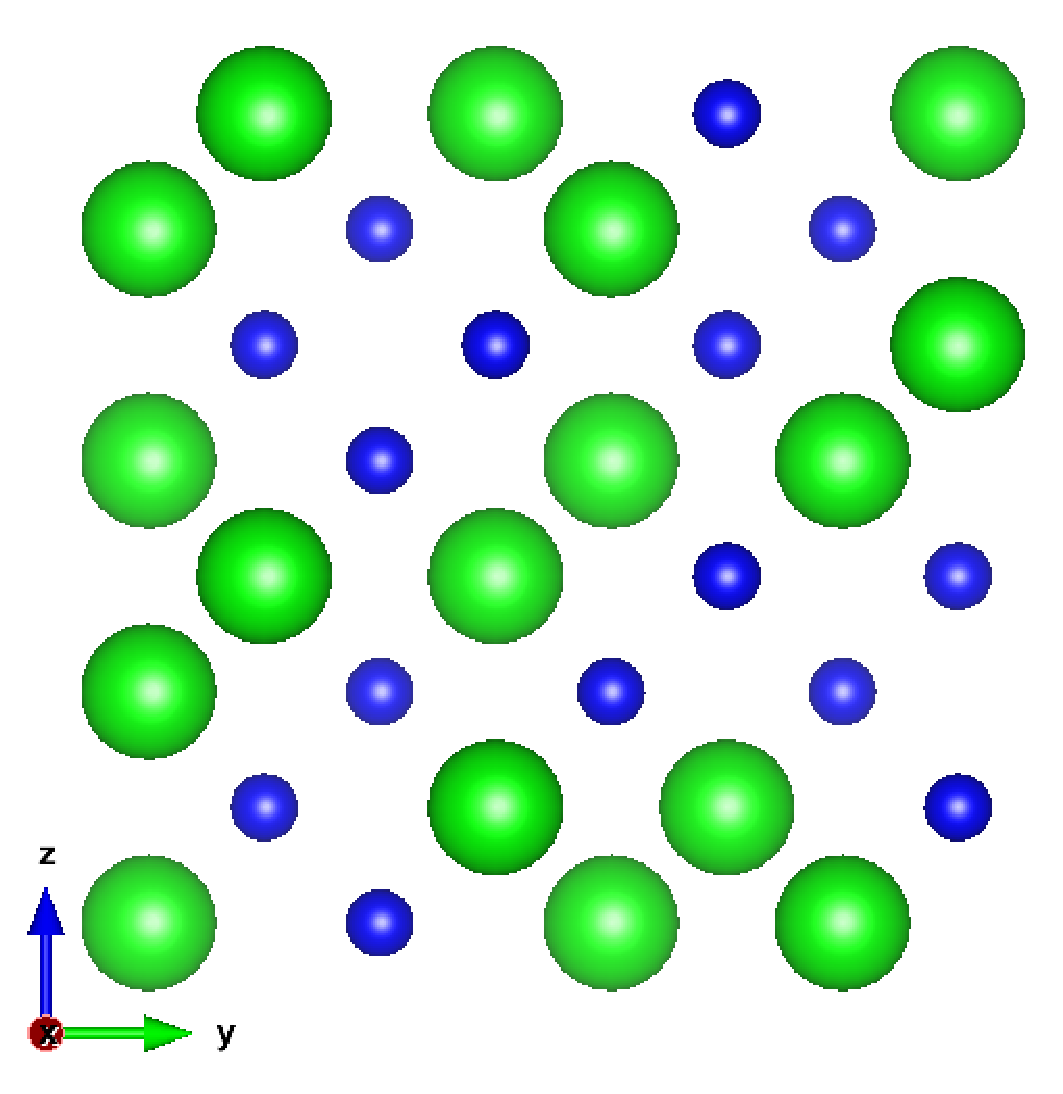
\includegraphics[scale=0.22]
{/home/jason/disorder/si/si_conv_2x2x2_disorder-2.eps}
\subfigure{(b)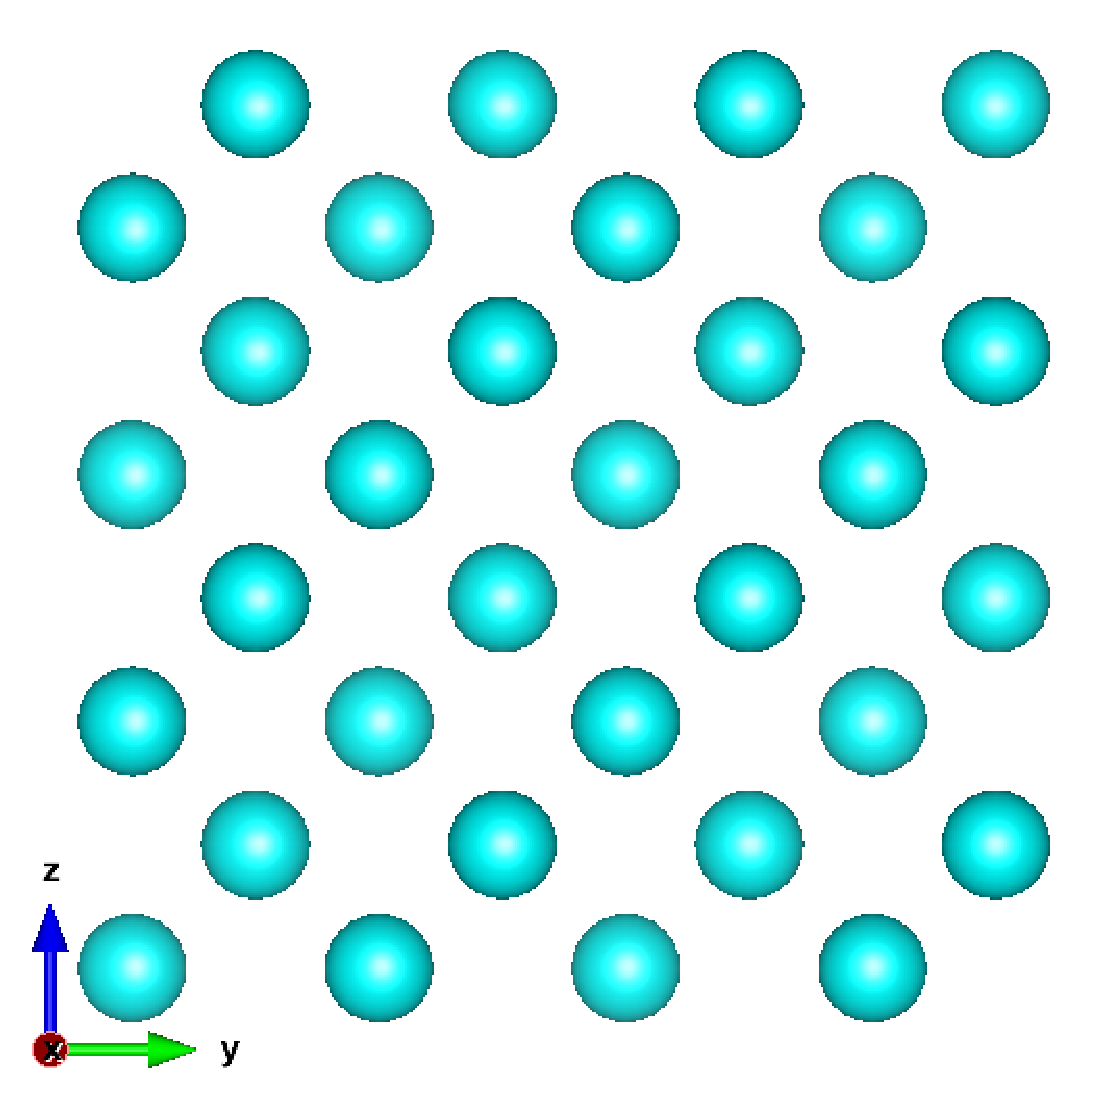
\includegraphics[scale=0.22]
{/home/jason/disorder/si/si_conv_2x2x2_perfect-2.eps}}}}
\vspace*{0mm}
\end{center}
\caption{\label{F:supercells} 
(a) view of an explicitly disoredered supercell of 
Si and ``heavy'' Si ([100] direction into the paper).
\cite{momma_vesta:_2008} 
(b) view of the equivalent VC supercell 
with an average
mass of the explicitly disordered Si and ``heavy'' Si supercell 
(b). 
Sphere size represents 
increasing mass 
only, no bond disorder is considered. 
In this work, calculations for LJ Ar and SW Si which use the VC 
approximation 
are based off of the conventional cubic unit cells 
(Section \ref{S:Calculation}) 
}
\end{figure}

%--------------------------------------------------------------------------


%--------------------------------------------------------------------------
\subsection{\label{S:Calculation}Calculation and Simulation Details}
%--------------------------------------------------------------------------

Perfect and explicitly disordered lattice supercells are generated 
with atomic positions 
based on LJ argon's FCC ($n=4$) and silicon's diamond-FCC ($n=8$) 
crystal structure, where $n$ is the number of atoms 
in the unit cell.   
Supercells are built cubically with size $N_0$, where $N_0$ refers to the 
number of repetitions of the unit cell in all 3 
spatial directions. Supercells up to size $N_0 = 12$ 
(6096 atoms) are used for the LJ argon calculations. For SW silicon, 
$N_0 \le 10$ (SW silicon, 8000 atoms) are used for 
the MD-based NMD methods, and $N_0 \le 42$ for MD-based GK and VC-ALD 
(see Appendix \ref{A:Finite Simulation-Size}).  

Disorder is created by randomly specifying the masses of the atoms 
on the lattice. 
The composition of the lattices is labeled by $m^i_{1-c}m^j_{c}$,  
where $m^i=1$ and $m^j=3$ in 
LJ units for argon and $m^i=m_{Si}$ and $m^j=2.6m_{Si}$ 
for SW silicon and ``heavy silicon'' (mass of germanium). 
For SW silicon, the lattice constant $a=5.43 \AA$ is used 
for all calculations, which brings the GK thermal conductivty 
predictions at 300K\cite{goicochea_thermal_2010,he_lattice_2012} 
into better agreement with VC-ALD
\cite{sellan_cross-plane_2010} for bulk SW silicon.
For LJ argon, supercells are built using 
the zero-pressure finite-temperature lattice constants, 
which are $a=1.556$ ($T$=10 K) and 
and $a=1.580$ ($T$=40 K) in LJ units.\cite{mcgaughey_phonon_2004} 
For LJ argon, the variation of lattice constant 
with composition is small and ignored.(cite) 
The amorphous LJ phase was created by liquifying the crystal 
and instantly quenching by removing all kinetic energy.  The resulting 
structure was then energy minimized and annealed in an NPT ensemble at 
zero pressure and $T=10$ K.(cite lammps)) 
The effective zero-pressure lattice constant  
of the amorphous phase at T=10K, based on the atomic 
density, is slightly larger 
($a = 1.585$).\cite{mcgaughey_phonon_2004}  

The MD simulations were performed by equilibrating in a NVT (constant 
number of atoms N, volume V, and temperature T) ensemble before 
calculating atomic positions and velocities in a NVE 
(constant number of 
atoms N, volume V and energy E) ensemble.(cite)  
Statistical averaging is accomplished 
using 10 simulations with different initial conditions. MD simulation 
time steps of 
4.285 and 0.5 fs were used for LJ argon and SW silicon. 
For the NMD method (Section \ref{S:From VC Gamma}), 
the atomic positions 
and velocities were sampled at a rate dictated by the highest vibrational 
frequencies in the system, which can be estimated from harmonic lattice 
dynamics calcualtions (Section \ref{S:VC Gamma DOS}). 
For the GK method, the heat current 
was computed every 10 time steps. It is important to note that the same 
atomic trajectories are used for the NMD and GK methods. 

%--------------------------------------------------------------------------
\section{\label{S:Vibrational}
Vibrational Mode Properties in Alloy Systems}
%--------------------------------------------------------------------------

%--------------------------------------------------------------------------
\subsection{\label{S:VC Gamma DOS}VC and Gamma DOS}
%--------------------------------------------------------------------------

In this section, we examine the effect of explicit disorder by computing 
the density of states (DOS, D$(\omega)$) for vibrational modes of  
disordered lattice supercells and their 
equivalent VCs. The frequencies 
are computed using harmonic lattice dynamics calculations with the package 
GULP.\cite{gale_general_2003} For the 
VC, the allowed wavevectors are set by $N_0$. For the disordered 
supercells,
the only allowed wavevector is the gamma-point (i.e., $\pmb{\kappa}=0$). 
The DOS for the VC and the explicitly disordered supercells 
(referred to herein as Gamma) are shown in Fig. \ref{F:DOS}. 
The VC and Gamma DOS 
agree at low frequencies, where the Debye approximation predicts 
$DOS \propto \omega^2$.(cite) The Debye approximation 
underpredicts the the DOS at moderate frequency, which is due to the 
non-linear dispersion.(cite Mermin)

SiGe DOS predictions

The increasing lattice 
mass with increasing concentration for the VC reduces  
the frequencies. The increasing lattice 
mass for the Gamma modes also reduces the frequencies.
The effect of expicit disorder is seen at high frequencies by a 
broadening and a shift of the DOS to higher frequencies 
because of the explicit use of light atoms in the supercell. 
Duda et al 
observed similar high-frequency broadening effects in model LJ alloys.
\cite{duda_reducing_2011} 
Similar agreement at low frequencies was found in \emph{ab initio} 
predictions 
for Si$_c$Ge$_{1-c}$,\cite{garg_role_2011} while Bouchard showed similar 
continuous behavior at low frequency for 
a-Si$_c$Ge$_{1-c}$.\cite{bouchard_vibrational_1988} 

%--------------------------------------------------------------------------
\begin{figure}
\begin{center}
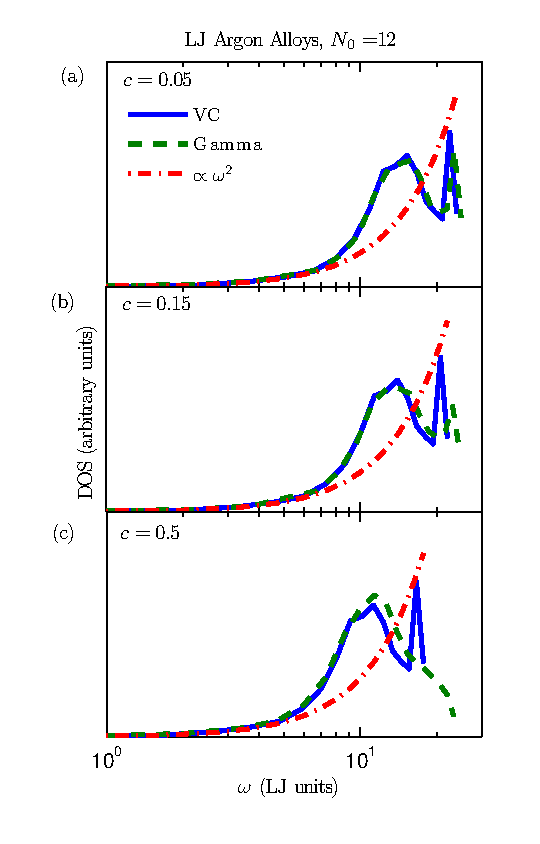
\includegraphics[scale=1.0]
{/home/jason/disorder/lj/alloy/lj_alloy_dos_c05-5_5.eps}
\vspace*{-5mm}
\end{center}
\caption{\label{F:DOS} Density of states (DOS) 
for modes calculated using the LJ FCC  
VC versus an explcitily mass disordered LJ FCC supercell 
(labeled Gamma) with varying mass concentration $c$. 
VC and Gamma show similar low frequency behavior for all $c$. 
For increasing $c$, the frequencies of both VC 
and Gamma decrease, while the high frequency DOS for Gamma spreads and  
reaches up to a higher maximum frequency because of the explict disorder. 
The size of these supercells is $N_0 = 12$ 
(see Section \ref{S:Calculation}).
}
\end{figure}
%--------------------------------------------------------------------------

%--------------------------------------------------------------------------
\subsection{\label{S:Dispersion}Dispersion and Group Velocity}
%--------------------------------------------------------------------------

%--------------------------------------------------------------------------
\subsubsection{\label{S:From VC}From Virtual Crystal}
%--------------------------------------------------------------------------

The group velocity vector in a VC is the gradient of the dispersion curves, 
\begin{equation}\label{EQ:Dynamical}
v_{g,\mathbf{n}}\kv = \frac{\partial \omega\kv}{\partial \pmb{\kappa}}.
\end{equation}
We calculate the group velocities for the VC  
using finite differences  
and quasi-harmonic lattice dynamics.\cite{mcgaughey_phonon_2006}

Except for the three 
acoustic branches (2 transverse, 1 logitudinal), there is not an 
accepted method to predict the effective group velocity of a 
vibrational mode in a disordered system, although there have been 
attempts.
\cite{cahill_lattice_1988,duda_reducing_2011,donadio_atomistic_2009,
he_heat_2011,he_thermal_2011} 
In the Cahill-Pohl (CP) model, the group velocity of all disordered 
modes is the sound speed, $v_s$.\cite{cahill_lattice_1988} 
Dispersion for a model disordered 1D system demonstrated   
the reduction of the frequency-dependent group velocities due to the 
zone-folding effect.\cite{duda_reducing_2011} By predicting the 
plane-wave character of vibrational modes, the structure factor of 
explicity disordered modes can be used to asses the 
applicability of the VC approximation.(cite)

%--------------------------------------------------------------------------
\subsubsection{\label{S:From Structure Factor}
From Structure Factor of Gamma Modes}
%--------------------------------------------------------------------------

Calculating the structure factor of Gamma   
modes is a method to test for the plane-wave 
character of disordered modes at a particular wavevector and 
polarization. 
\cite{allen_diffusons_1999,feldman_numerical_1999} 
Feldman et al used the structure factor to predict an effective dispersion 
for a model of a-Si, but did not predict group velocities.
\cite{feldman_numerical_1999} 
Volz and Chen used the dynamic structure factor to predict the
dispersion of crystalline SW Si using MD simulation.
\cite{volz_molecular-dynamics_2000}

The structure factor is defined as\cite{allen_diffusons_1999} 
\begin{equation}\label{EQ:SLT}
S^{L,T}\kw = 
\sum_{\nu} E^{L,T}\kgv
\delta (\omega-\omega\kgv),
\end{equation}
where $E^{T}$ refers to transverse polarization and is defined as
\begin{equation}\label{EQ:EL}
E^L\kgv = 
\left|
\sum_{l,b} 
\hat{\mathbf{\kappa}} \cdot e\kgvba 
\EXP{i\pmb{\kappa}\cdot\mathbf{r}_0\ab{l=0}{b}} 
\right|^2
\end{equation}
and $E^{L}$ refers to logitudinal polarization and is defined as
\begin{equation}\label{EQ:ET}
E^T\kgv = 
\left|
\sum_{l,b} 
\hat{\mathbf{\kappa}} \times e\kgvba 
\EXP{i\pmb{\kappa}\cdot\mathbf{r}_0\ab{l=0}{b}} 
\right|^2.
\end{equation}
Here, $\mathbf{r}_0\ab{l=0}{b}$ refers to the atomic positions of the 
mass disordered atoms in the supercells, which are still spaitally ordered. 
Explicit disorder is accounted for in the mode frequencies $\omega\kgv$ 
and eigenvectors $e\kgvba$, which are calculated with 
$\mathbf{\kappa} = \mathbf{0}$. The structure factors for LJ argon alloys 
are plotted in Fig. \ref{F:SF} for wavevectors allowed by the VC. 

Physically, $S^{L,T}\kw$ represents  
the frequency spectrum required to create a wavepacket with a 
well-defined wavevector and polarization.
\cite{allen_diffusons_1999,feldman_numerical_1999} The details of the 
calculation are given in Appendix . 
For a perfect lattice, the 
structrue factor peaks are delta functions centered at the phonon mode 
frequencies, indicating they are pure plane-waves. 
With increasing disorder, the structure factor spreads in width in 
Fig. \ref{F:SF},  
particularly at high frequencies because the modes are no longer 
pure plane-waves. The spectral mode factors $E^{L,T}\kgv$ represent the 
plane-wave character of any given mode $\omega\kgv$. We find that 
individual modes cannot be assigned a unique wavevector using 
$E^{L,T}\kgv$, in agreement with similar results for a-Si.(cite) 

From Fig. \ref{F:SF}, 
an effective dispersion can be extracted by locating the peaks in the 
structure factors at neighboring VC wavevectors, where the 
effects of polarization, virtual mass, and 
anisotropic dispersion can be observed. 
As the lattice VC mass becomes larger,  
the peaks in the structure factor shift to lower frequencies. 
The peaks in the structure factor are at  
slightly 
higher frequencies than the VC predicted frequencies by 
up to only $\%5$. Similarly, good agreement is found with the disordered 
SW silicon lattices (not shown), while the structure factors are 
more complicated because of the optical modes. 
Because of this good agreement,  
we use the group velocities predicted by the VC dispersion for both
LJ argon and SW silicon 
with the VC-NMD and VC-ALD calculations for 
consistency and simplicity. We will examine 
the validity of this choice of group velocity in 
Section \ref{S:Diffusivities}. 
Well-defined peaks (see Appendix \ref{A:SF}) 
at all wavevectors are most likely due to the 
lattice structure of the disordered systems studied in this 
work. 
Typically, the structure factor for amorphous materials has well-defined 
peaks only for small wavevector.
\cite{allen_diffusons_1999,feldman_numerical_1999}   

%--------------------------------------------------------------------------
\begin{figure}
\begin{center}
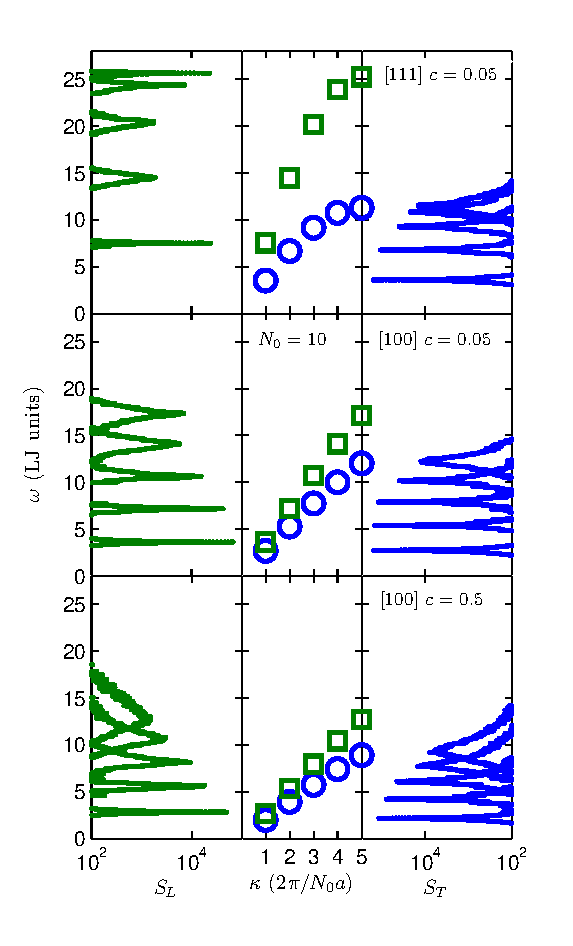
\includegraphics[scale=1.0]
{/home/jason/disorder/lj/alloy/lj_alloy_dsf_100_111-2.eps}
\vspace*{-5mm}
\end{center}
\caption{\label{F:SF} 
Left and Right Panels: 
The structure factor for logitudinal ($S_L$) 
and transverse ($S_T$) 
polarizations along high symmetry directions ([100], [110] 
where $\mathbf{\kappa}$ = $\pi/a[100]$ and $a$ is the 
lattice constant ) 
of the mass disordered LJ FCC supercells ($c=0.05,0.5$). 
For increasing 
mass disorder $c$, there is a decrease in the center of the peaks 
and an increase in the peak linewdiths. 
Center Panel:
The VC predicted dispersion at the same wavectors used to calculate 
$S_{L,T}$.
}
\end{figure}
%--------------------------------------------------------------------------

%--------------------------------------------------------------------------
\subsection{\label{S:Phonon Lifetimes}Lifetimes}
%--------------------------------------------------------------------------

%--------------------------------------------------------------------------
\subsubsection{\label{S:From VC Gamma}From VC-NMD and Gamma-NMD}
%--------------------------------------------------------------------------

As an alternative to the VC-ALD models for predicting phonon lifetimes, 
which are discussed in the next section,  
we first use the normal mode decomposition (NMD) method.
\cite{ladd_lattice_1986,turney_predicting_2009} 
NMD maps the 
atomic trajectories (positions and velocities) of atoms in an MD 
simulation onto the vibrational normal mode coordinates,(cite)
\begin{equation}\label{E:q_HLD}
\begin{split}
q\kvt=&\SUM{0}{}\sqrt{\frac{m_b}{N}}u_{\alpha}\lbt e^*\kvba
\EXP{i\pmb{\kappa}\cdot\mathbf{r}_0\ab{l}{0}}
\end{split}
\end{equation}
and
\begin{equation}\label{A:E:qdot_HLD}
\begin{split}
\dot{q}\kvt{}{}{}=&\SUM{0}{}\sqrt{\frac{m_b}{N}}\dot{u}_{\alpha}
\lbt e^*\kvba\EXP{i\pmb{\kappa}\cdot\mathbf{r}_0\ab{l}{0}}.
\end{split}
\end{equation}
where $\mathbf{r}_0\ab{l}{0}$ are the equilibrium positions of the atoms 
in the $l$th unit cell of the lattice supercell under the VC 
approximation. 
The total energy of a given vibrational mode is 
\begin{equation}\label{A:E:qdot_HLD}
\begin{split}
E\kvt = \frac{\omega\kv}{2} q\kvt^*q\kvt + 
\frac{1}{2}\dot{q\kvt}^*\dot{q\kvt}
\end{split}
\end{equation}

We perform NMD using the frequencies and eigenvectors 
from both the VC ($\omega\kv$, $e\kvba$) and the Gamma supercell 
($\omega\kgv$, $e\kgvba$). 
The trajectories from 
these MD simulations are also used in the GK method 
(Section \ref{S:Thermal Conductivity}).

The normal vibrational mode lifetime is predicted using 
\begin{equation}\label{EQ:tau_nmd}
\tau\kv = \int_{0}^{\Tau}
\frac{<E\kvt E\kvzero>}{ <E\kvzero E\kvzero> }dt,
\end{equation}
where the upper integration limit is set by  
the specifications of the MD simulation.(cite) This method for predicting  
lifetimes is able to handle the more complex behavior of the VC-NMD  
energy autocorrelations due to the disorder, which 
generally follow exponential decay  
(see Appendix \ref{A:NMD XCORR}). This choice is an approximation which  
also makes it difficult to predict a phonon frequency, so we use the 
VC predicted frequency for all VC-NMD predictions to compare with 
VC-ALD (Section \ref{S:Diffusivities}).

The lifetimes predicted using VC-NMD and Gamma-NMD  
are shown in Fig. \ref{F:VC Gamma life} for LJ argon alloys. 
The range of frequencies of the modes for 
VC-NMD and Gamma-NMD differ slightly  
which is due to differences in the DOS (Fig. \ref{F:DOS}). 
For small intervals of frequency, there are a wider range of 
predicted lifetimes for Gamma-NMD. This is because there is no symmetry 
averaging of the mode properties, which is possible for the VC.
Lifetimes predicted by both VC-NMD and Gamma-NMD show scalings with 
frequency of $\omega^{-2}$ at low frequency and $\omega^{-4}$ and 
even faster for mid-range frequencies (Fig. \ref{F:DOS}). 
In general, the lifetimes predicted by both VC-NMD and Gamma-NMD  
are larger than the Ioffe-Regel (IR) limit,
\cite{taraskin_determination_1999} 
\begin{equation}\label{EQ:IR}
\tau = \frac{2\pi}{\omega}.
\end{equation}
The physical interpretation of the IR limit is that of a mode which 
scatters in a time equal to its oscillation period, which seems to 
be a good lower-limit for the lifetimes predicted by VC-NMD and Gamma-NMD 
for LJ argon (Fig. \ref{F:VC Gamma life}) 
and VC-NMD for SW silicon (Fig. \ref{F:Dph_si}(a)). 

The behavior at the highest frequencies, 
where $\tau \propto constant$, is seen for both VC-NMD and Gamma-NMD, 
except at $c=0.5$ for VC-NMD.  
Since the existence of this 
characteristic (thought not exactly minimum) lifetime for LJ argon is 
demonstrated by both VC-NMD and Gamma-NMD, it is physically 
meaningful. There is, however, no theoretical 
prediction of this high-frequency behavior of the mode lifetime.
\cite{kittel_interpretation_1949,cahill_lattice_1988,
graebner_phonon_1986} This 
plateau of lifetimes at high-frequency is not seen for SW 
silicon (Fig. \ref{F:Dph_si} a). 

Overall, good agreement is seen in the predicted lifetimes from VC-NMD and 
Gamma-NMD both in magnitude and trends. The use of the VC normal modes 
is an approximation which becomes worse as the concentration is increased 
(Appendix ). The only approximation associated with Gamma-NMD is the use  
of the harmonic lattice dynamics predicted frequencies and eigenvectors 
to map the atomic trajectories from the fully anharmonic MD simulations.
(cite) 
Based on the good agreement with Gamma-NMD, the 
lifetimes predicted by VC-NMD are used along with the VC predicted 
group velocities to 
predict thermal conductivity in Section \ref{S:Thermal Conductivity}. 

%--------------------------------------------------------------------------
\begin{figure}
\begin{center}
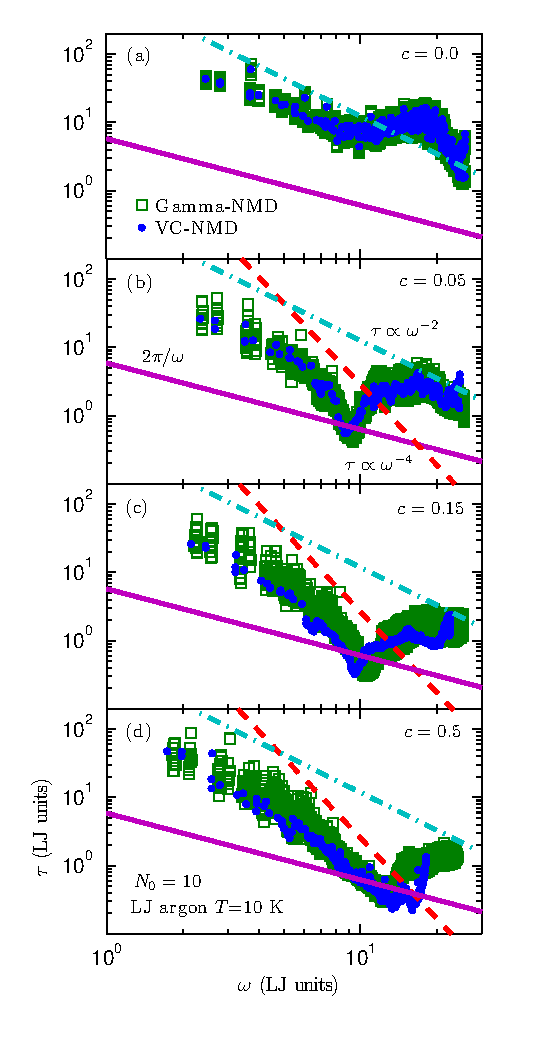
\includegraphics[scale=1.0]
{/home/jason/disorder/lj/alloy/lj_alloy_nmd_vc_gamma_life-3.eps}
\vspace*{-5mm}
\end{center}
\caption{\label{F:VC Gamma life} Lifetimes predicted using VC-NMD 
and Gamma NMD from MD simulations of mass disordered lattice supercells 
(Section \ref{S:From VC Gamma}). 
Both $\omega^{-2}$ and $\omega^{-4}$ scalings can be observed 
at low frequencies, which are predicted by the peturbative models used 
for VC-ALD (Section \ref{S:From VC-ALD}). 
For both VC-NMD and Gamma NMD, most mode 
lifetimes are greater than the Ioffe-Regel limit $\tau = 2\pi/\omega$. 
\cite{taraskin_determination_1999}
While there is more ``noise'' in the Gamma-NMD data 
(Section \ref{S:From VC Gamma}), the lifetime magnitudes and 
trends agree well, an important consideration when comparing VC-NMD and 
VC-ALD in Fig. \ref{F:Dph_lj} .
}
\end{figure}
%--------------------------------------------------------------------------


%--------------------------------------------------------------------------
\subsubsection{\label{S:From VC-ALD}From VC-ALD}
%--------------------------------------------------------------------------

Assuming initrinsic and disorder scattering mechanisms 
to operate independently, the 
effective phonon lifetime can be found using Matthiessen's rule(cite),
\begin{equation}\label{EQ:Matthiessen}
\frac{1}{\tau\kv} = \frac{1}{\tau_{p-p}\kv} + \frac{1}{\tau_{p-d}\kv},
\end{equation}
where $\tau_{p-p}\kv$ accounts for intrinsic phonon-phonon scattering 
and $\tau_{p-d}\kv$ accounts for defect scattering.

Phonon-phonon scattering ($\tau_{p-p}\kv$) is typically treated 
using anharmonic perturbation theory (ALD) including only three-phonon 
processes.\cite{turney_predicting_2009,garg_role_2011,tian_phonon_2012} 
It has been demonstrated that the effects of higher order phonon 
processes become important at high temperatures.
\cite{ecsedy_thermal_1977,turney_predicting_2009} 
In this work, the intrinsic phonon lifetimes $\tau\kv_{p-p}$ 
are predicted using the method described in
\cite{turney_predicting_2009}, with all classical expressions to remain 
consistent with the classical MD-based methods NMD and GK. 

Using harmonic perturbation theory, Tamura derives a general expression 
for mass point defect scattering.\cite{tamura_isotope_1983} 
By considering the symmetry properties of the FCC lattices 
considered in this work (Section \ref{S:Calculations}), 
it can be shown that\cite{tamura_isotope_1983}
\begin{equation}\label{EQ:taud_dos}
\begin{split}
1/\tau_{d}\kv =\frac{\pi}{2} g_2 \omega^2\kv D(\omega), 
\end{split}
\end{equation}
where 
$D(\omega)$ is the density of states (Section \ref{S:VC Gamma DOS}) and 
$g_n = \sum_\mu c^{\mu}(1-m^{\mu}/\bar{m}^{\mu})^n$.
Here, $c^\mu$ is the concentration, 
$m^\mu$ is the mass of the $\mu$-th species 
and $\bar{m}^{\mu}$ is the average mass. Bond disorder 
can be accounted for using a similar expression with an average
atomic radius or suitable scattering cross-section.
\cite{klemens_scattering_1955,klemens_thermal_1957} 
For the binary LJ argon and SW silicon alloys considered, 
there is one atom type in the unit cell  
with $\mu=i,j$, so that the alloying atom labeled by $m^i_{1-c}$ 
can be considered to be an ``isotope'' of atom labeled 
$m^j_{c}$.  This convention is appropriate because of the 
perturbative approach used to derive Eq. () , while we consider 
large disorder.\cite{tamura_isotope_1983} 
To calculate the disordered lifetimes $\tau\kv_{d}$ (Eq. ), 
it is necessary to broaden 
the $\delta$ function using a Lorentzian function.[1] 
footnote[1]
For all calculations, the Lorentzian was broadened using a value of 
$100\delta_{\omega,avg}$ (Section \ref{S:SF}). 
For the system sizes here, 
the results do not differ significantly 
if this broadening value is varied manually or  
by increasing system size ($N_0$).

At low frequencies where the density of states is Debye-like 
($D(\omega) \propto \omega^{2}$), Fig. \ref{F:DOS}), 
$\tau_{p-p}\kv$ follows a scaling due to both normal ($B_1\omega^{-2}$) 
and umklapp ($B_2\omega^{-2}$) 3-phonon scattering processes, where the 
constants $B_1$ and $B_2$ are typically fit to experimental data.(cite) 
From Fig. \ref{F:VC Gamma life} and \ref{F:Dph_lj} a , 
the scaling $\tau \propto \omega^{-2}$ can be 
observed  
in the VC-NMD, Gamma-NMD and VC-ALD predicted results. 
Under the Debye-approximation , 
the phonon scattering due to mass point-defects 
is given by $A\omega^{-4}$, where $A$ is a constant related to the unit 
cell volume, branch-averaged group velocity, and disorder coupling strength 
($g_2(b)$ in Eq. above). 
The frequency dependence ($\omega^4$) is the same as 
Rayleigh scattering, which is valid at low frequency and observed 
in both the NMD (Fig. \ref{F:VC Gamma life}) and ALD 
(Fig. \ref{F:Dph_lj}) predicted lifetimes. 
VC-ALD does not predict the behavior of the lifetimes at high frequency 
for LJ argon, $\tau \propto constant$. The thermal conductivity of 
LJ argon alloys is dominated by high frequency modes 
(Fig. \ref{F:Dph_lj} c).(cite)  
For SW silicon alloys, the thermal conductivity is dominated by 
low-frequency modes, while the high frequency discrepancy is 
not observed using VC-NMD and VC-ALD (Fig. \ref{F:Dph_si} c). 
% The disorder 
% scattering scaling is expected to fall off faster than $\omega^{-4}$ 
% when $D(\omega)$ grows faster than the Debye scaling of 
% $\omega^{2}$ (Fig. , Section ). 
% The lifetimes do fall off faster $\omega^{-4}$ for the 
% mass disordered LJ FCC supercells for a narrow range of 
% frequencies near $\omega = 10$ in Fig. for $c=0.05,0.15$, 
% but seem to follow more closely $\omega^{-4}$ for $c=0.5$. 

The Tamura theory was developed to predict the reduction of lifetimes 
in isotopic Ge, which is only perturbatively disordered. 
The terms $g_n$ are  
coupling terms which define the strength of the disorder and the 
importance of n-order interactions in the Tamura theory.  
With increasing disorder, 
the importance of higher-order ($n > 2$) terms in the 
Tamura theory can be estimated by $g_n|I(\omega)|^{n-2}/g_{n-1}$, 
where $I(\omega)$ is related to the DOS.\cite{tamura_isotope_1983} 

For isotopically-disordered Ge, the higher-order contributions 
$g_n|I(\omega)|^{n-2}/g_{n-1}$ were estimated to be negligible for all 
frequencies.\cite{tamura_isotope_1983} 
For LJ argon and the large concentrations and mass ratios considered 
in this work, the terms 
$g_n|I(\omega)|^{n-2}/g_{n-1}$ are order 1 and larger at high 
frequencies. It is possible that 
higher-order interactions in the Tamura theory 
is responsible for the 
discrepancy of the lifetimes predicted by VC-NMD and Gamma-NMD 
versus VC-ALD at high frequency.
For SW silicon alloys the higher-order terms are also large, while 
good agreement is observed at high frequencies for VC-NMD and VC-ALD 
(Fig. \ref{F:Dph_si}).

% NOT USED:
% $c=0.001$ $g_3 = -0.0079$, $g_4 = 0.0158$,
% $c=0.001$ $g_3 = -0.0079$, $g_4 = 0.0158$,
% $c=0.01$ $g_3 = -0.073$, $g_4 = 0.142$,   
% $c=0.15$ $g_3 = -0.325$, $g_4 = 0.441$
% $c=0.5$ $g_3 = 0.0$, $g_4 = 0.0625$

%--------------------------------------------------------------------------
\subsection{\label{S:Diffusivities}
Diffusivities}
%--------------------------------------------------------------------------

In the classical harmonic limit, where the specific heat 
$c_p\kv = k_{\mathrm{B}}$, 
a vibrational mode's contribution to thermal 
conductivity is determined by the mode thermal diffusivity. For 
phonons, the thermal diffusivity is 
\begin{equation}\label{EQ:Dph}
D_{ph,\mathbf{n}}\kv = \pmb{v}_{g,\mathbf{n}}\kv \tau\kv.
\end{equation}
For VC-NMD and VC-ALD, $\pmb{v}_{g,\mathbf{n}}\kv$ is calculated 
from the VC dispersion (Section \ref{S:From VC}) so any differences in 
thermal diffusivity comes from the predicted lifetimes. The lower limit 
for phonon thermal diffusivity is 
$D_{ph,\mathbf{n}}\kv \approx 0$ since the 
group velocities can approch 0 for modes such as optical 
and those near the Brioullin zone boundaries.(cite)

In disordered systems,  
modes can transport heat by harmonic coupling due to disorder 
in the Allen-Feldman (AF) theory of diffusons.\cite{allen_thermal_1993} 
In the high-scatter (HS) limit,(cite) 
the AF diffusivity of each mode is
\begin{equation}\label{EQ:M:k_HS}
D_{AF,HS} = \frac{1}{3} v_s a,
\end{equation}
and the AF thermal conductivity prediction is
\begin{equation}\label{EQ:M:k_HS}
k_{AF,HS} = \frac{k_{B}}{V_b}b v_s a,
\end{equation}
where $V_b$ is the volume of the unit cell, $v_s$ is the 
branch-averaged sound speed, and $a$ is the lattice constant.
\cite{cahill_lattice_1988} 
The Cahill-Pohl (CP) HS limit  
differs from the AF,HS model by a factor of approximately $\%20$.
\cite{cahill_lattice_1988} 
The physical interpretation is all vibrational 
modes transport heat at the sound speed 
and scatter with a mean free path of the lattice spacing. 

As seen in Fig. \ref{F:Dph_lj} and \ref{F:Dph_si}, 
VC-NMD and VC-ALD predict a significant 
number of modes with  
$D_{ph}\kv < D_{AF,HS}$ for both LJ argon and SW silicon. 
This can lead to an underprediction of the 
total thermal conducitvity. The diffusivity of these 
modes can be adjusted such that any mode with $D_{ph} < D_{AF,HS}$ is 
given $D_{ph} = D_{AF,HS}$.  The result of this adjustment, 
referred to as VC-NMD* and VC-ALD*, is examined 
in the thermal conductivity predictions in Section 
\ref{S:Thermal Conductivity}.

While AF,HS model assumes a mode-independent thermal diffusivity, 
the AF theory is capable of predicting the mode specific 
diffusivities.\cite{feldman_thermal_1993,feldman_thermal_1993,
feldman_numerical_1999,shenogin_predicting_2009} 
In the harmonic AF theory, mode diffusivities 
typically diverge as $\omega \rightarrow 0$ because
the vibrational modes are long-wavelength plane waves  
that weakly scattered by the disorder.
\cite{sheng_introduction_2006,vitelli_heat_2010}
\footnote[1]
{For the disordered lattices studied 
in this work for $c\le0.15$, the predicted $k_{AF}$ is strongly 
system size dependent, indicating this diverging behavior. 
For LJ argon alloys at $c=0.5$, the divergence with system size is 
small for the range of system size studied ($N_0=4$ to $N_0=12$), 
where $k_{AF}/k_{GK} = 0.93$ for $N_0=12$.} 
The mode-specific thermal diffusivities for the LJ argon amorphous phase 
are shown in Fig. \ref{F:AF}.
\footnote[2]{For a finite system, the AF theory 
requires a broadening in frequency to predict the mode-specific thermal 
diffusivities.  We use a Lorentzian broadening with a width of 
$\delta_{\omega,avg}$, see Section \ref{S:SF}.} 
Modes with significant 
contribution to thermal transport can be modeled using a mode-independent 
diffusivity of approximately $D_{AF,HS}$.  
Also shown are the AF predicted thermal 
diffusivities for the explicitly disordered superlattice and $c=0.5$. 
While the AF theory is divergent in the low-frequency limit for lattices,  
the finite system size limits the thermal diffusivities of the lowest 
frequencies. The thermal diffusivity of all 
modes in the explicitly disordered lattice supercell are 
larger than $D_{AF,HS}$, except 
at the highest frequencies where they tend to zero as in the amorphous 
phase.(cite)\footnote[3]{Analysis of these high-frequency 
modes shows that they are locons, 
modes which are spatially localized in the Anderson sense. 
Feldman et al showed that the thermal 
diffusivities in a-Si show a sharp breakpoint at the on-
set of localized states, where it tends to zero exponentially. 
The correct 
length scale associated with these modes is the mode correlation 
length(cite), whose uppper bound is the size of the simulation domain.} 
This result supports the plausible lower-bound, $D_{ph} \ge D_{AF,HS}$. 

Predictions from model 
disordered systems demonstrates the existence of a plateau of the 
thermal diffusivity, 
which is consistent with the minimum phonon mean-free path hyopthesis.
\cite{sheng_heat_1991} 
A minimum vibrational mean free path is used in most models of thermal 
transport in disordered materials.
\cite{kittel_interpretation_1949,cahill_lattice_1988,
graebner_phonon_1986} However, the concept of 
a vibrational mean free path is only valid for low-frequency propagating 
modes in disordered systems.\cite{feldman_numerical_1999} The more 
fundamental proprety is the vibrational mode lifetime.
\cite{taraskin_determination_1999}  

For disordered systems it is only possible to assign a 
unique lifetime and group velocity to a vibrational mode 
only in the low-frequency, propagating limit.
\cite{feldman_numerical_1999,xu_energy_2009} 
This implies that the VC predicted group velocities, particluarly 
for $v_g\kv << v_s$, are an underprediction of the representative 
velocity scale for the thermal diffusivity of high-frequency modes 
in the disordered lattice.

VC-NMD predicts lifetimes which 
are generally larger than the IR limit (Eq. ) 
for both LJ argon and SW silicon alloys.   
VC-ALD predicts essentially monotonically 
decreasing lifetimes with increasing frequency for both LJ argon and SW 
silicon (Fig. \ref{F:Dph_lj} a and \ref{F:Dph_si} a). 
Because VC-NMD and VC-ALD 
use the same predictions for $v_g\kv$, the phonon mode 
diffusivities $D_{ph}\kv$ are underpredicted for 
VC-ALD compared to VC-NMD for LJ argon alloys. 
There are thus 2 underpredictions to consider 
when predicting the thermal conductivities in predictions: 
underprediction 
of the thermal diffusivity assuming the VC group velocities for 
VC-NMD and VC-ALD, and the underprediction of the mode lifetimes for 
LJ argon alloys by 
the VC-ALD perturbative models. 

% NOT USED:
% energy transport in jammed sphere packings\cite{xu_energy_2009}
% heat transport in model jammed solids\cite{vitelli_heat_2010}

%--------------------------------------------------------------------------
\begin{figure}
\begin{center}
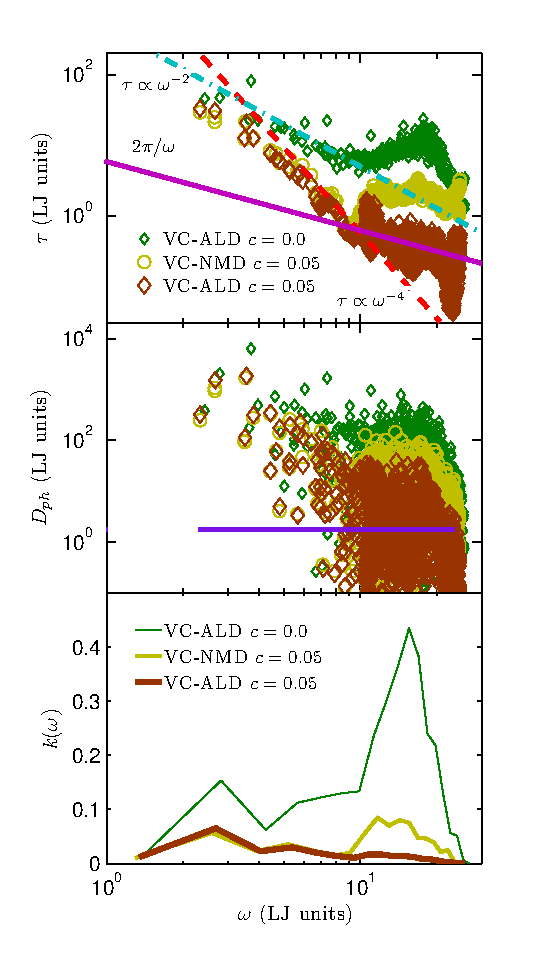
\includegraphics[scale=1.0]
{/home/jason/disorder/lj/alloy/af_nmd_ald_tau_diff_kw_c05_3-3.eps}
\vspace*{-5mm}
\end{center}
\caption{\label{F:Dph_lj} (a) predicted lifetimes for VC modes using 
VC-NMD and VC-AlD for LJ argon. 
(b) predicted VC mode thermal diffusivities, compared  
to the AF,HS limit. (c) the thermal conducitivty frequency spectrum, 
which is peaked at high frequency, in contrast to SW silicon (Fig).}
\end{figure}
%--------------------------------------------------------------------------

%--------------------------------------------------------------------------
\begin{figure}
\begin{center}
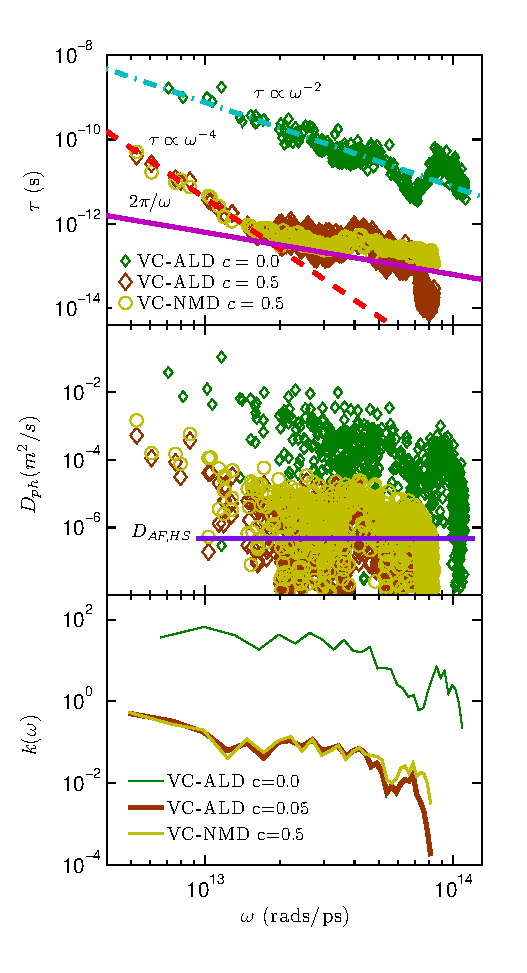
\includegraphics[scale=1.0]
{/home/jason/disorder/si/alloy/af_nmd_ald_tau_diff_kw_c5.eps}
\vspace*{-5mm}
\end{center}
\caption{\label{F:Dph_si} (a) predicted lifetimes for VC modes using 
VC-NMD and VC-AlD for SW silicon. 
(b) predicted VC mode thermal diffusivities, compared  
to the AF,HS limit. (c) the thermal conducitivty frequency spectrum, 
which is peaked at low frequency, in contrast to LJ argon 
(Fig. \ref{F:Dph_lj}). }
\end{figure}
%--------------------------------------------------------------------------

%--------------------------------------------------------------------------
\begin{figure}
\begin{center}
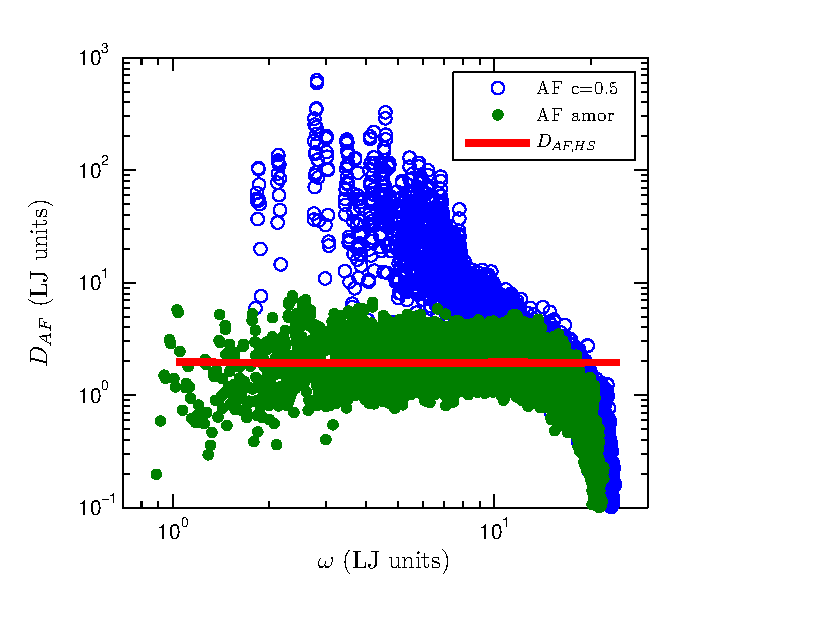
\includegraphics[scale=1.0]
{/home/jason/disorder/lj/alloy/af_c5_amor_DAF_kw_2.eps}
\vspace*{-5mm}
\end{center}
\caption{\label{F:AF} AF theory predictions of disorded mode  
thermal diffusivities for LJ argon disorded lattice supercell and 
amorphous phase. The mode thermal diffusivities predicted for the 
disorded lattice supercell are all finite, except at the highest 
frequency where they tend to 0 as in the amorphous phase. }
\end{figure}
%--------------------------------------------------------------------------


%--------------------------------------------------------------------------
\section{\label{S:Thermal Conductivity}Thermal Conductivity Predictions}
%--------------------------------------------------------------------------

The thermal conductivity can be predicted using the mode properties 
predicted by the VC-NMD and VC-ALD 
methods.  Given the discussion of the preceeding section, 
it is necessary to implement a third method 
for predicting thermal condudctivity. 
We choose the equilibirum MD-based green-kubo (GK) method.(cite) 
This method 
does not predict any mode-specific properties, and is thus a system-level 
prediction. Thermal conductivity predicted by GK 
has been shown to capture the effects of whatever scattering 
meachanisms are 
present in the MD simulation without any assumptions (other than 
those that come with the classical nature of the MD siulation).(cite) 
Details of the GK and MD simulations are given in Appendix . 
For LJ argon, bulk thermal conductivity predictions are made for 
VC-NMD, VC-ALD and GK (Fig. \ref{F:cond_lj}). 
For SW silicon, bulk thermal conductivity 
predictions can only be made for VC-ALD and GK (Fig. \ref{F:cond_si}) 
because of the 
limited system size used for VC-NMD (see Appendix ). 

For LJ argon, VC-NMD and VC-ALD underpredict the thermal 
conductivity compared to GK. 
The underprediction is only modest for VC-NMD, on the order of 
$20\%$ or less for all $c$. By adjusting the mode diffusivity as 
suggested 
in Section \ref{S:Diffusivities}, 
the thermal conductivtiy predicted by VC-NMD$^*$ is 
brought 
into agreement with GK by approximately $10\%$ or less for all $c$. 
Combined with the high-scatter limit, the VC-NMD predicted thermal 
diffusivities are a fair representation of the explicitly 
disordered modes present in the MD simulation when.

The VC-ALD method underpredicts the thermal conductivity of LJ argon 
alloys, 
where 
the underprediction is worst for $c=0.05$, $k_{VC-ALD} / k_{GK} = 0.56$ 
(error bars are on the order 
of the large symbol sizes in Fig. \ref{F:cond_lj}). 
By applying the high-scatter limit 
adjustment VC-ALD$^*$, the thermal conductivities are brought into 
marginally 
better agreement, worst for $c=0.05$, $k_{VC-ALD^*} / k_{GK} = 0.65$. 

The failure of the VC-ALD method can be demonstrated further 
by moving to higher temerpature $T=40$ K in Fig. \ref{F:cond_lj} a.
The beginning breakdown of the intrinsic phonon-phonon ($\tau_{p-p}\kw$) 
scattering model 
can be observed for $c=0.0$ at 
$T=40$ K (Fig. \ref{F:cond_lj} b), 
where ALD begins to overpredict compared to GK. 
This 
can be explained by the emerging importance of higher order (n$> 3$) 
n-phonon process at high temperatures.\cite{turney_predicting_2009} 
While the VC-ALD method begins to overpredict for $c=0.0$ 
at elevated temperature, 
it continues to underpredict for the alloys $c \ge 0.05$.  In fact, the 
thermal conductivity predictions for VC-ALD are at or slightly below the  
high-scatter limit $k_{AF,HS}$. 

The VC-ALD method fails to 
accurately predict the high-frequency mode thermal diffusivities for 
LJ argon alloys, which can be seen in the thermal conductivity 
spectrum Fig. \ref{F:Dph_lj} c.(cite) 
Since the group velocities are the same for VC-NMD and VC-ALD, 
this underprediction of the high-frequency thermal diffusivities is 
due to the underpediction of the high-frequency 
mode lifetimes (Fig. \ref{F:Dph_lj} a). 
At T=40 K, the thermal conductivity of the diffusivity adjusted 
VC-ALD$^*$ is only marginally improved compared to GK. 

For SW silicon, the thermal conductivities predicted by VC-ALD and GK 
are in better agreement, even without the adjustment VC-ALD$^*$. VC-ALD 
actually overpredicts by roughly $20\%$ for $c \ge 0.05$ compared to GK.
\footnote[4]
{The overprediction of thermal conductivity by VC-ALD 
may be related to the role of disorder in the ALD calculation.
\cite{garg_role_2011,turney_predicting_2009} While Garg et al found 
an overprediction of VC-ALD compared to experiment by a factor of two, 
the overprediction 
we observe in this work for SW silicon alloys is not as drastic.}   
For SW silicon alloys, the VC-ALD$^*$ adjustment  
increases the result from VC-ALD by about 1$\%$ because the contribution 
from high-frequency modes is only a few percent (Fig. \ref{F:Dph_si} c). 

% NOT USED:
% In SW silicon, the amorphous phase has significant contributions 
% from propagating modes which are considered to be phonons.(cite) Without 
% any detailed mode-by-mode analysis, comparing the thermal 
% conductivity predicted for the 
% SW silicon amorphous phase ($k_{GK} \approx$ 3 W/m-K (cite)) compared to 
% the HS limit, 
% $k_{AF,HS} = $0.5 W/m-K, demonstrates that there is significant 
% contribution from what can be considered propagating modes.(cite)  
% In fact, for a-Si, the mode diffusivities vary strongly as a function 
% of frequency,
% \cite{feldman_thermal_1993,feldman_numerical_1999,allen_diffusons_1999} 
% which has been used to explain the propagating 
% mode effects seen in a-Si thin films.\cite{he_heat_2011}

%--------------------------------------------------------------------------
\begin{figure}
\begin{center}
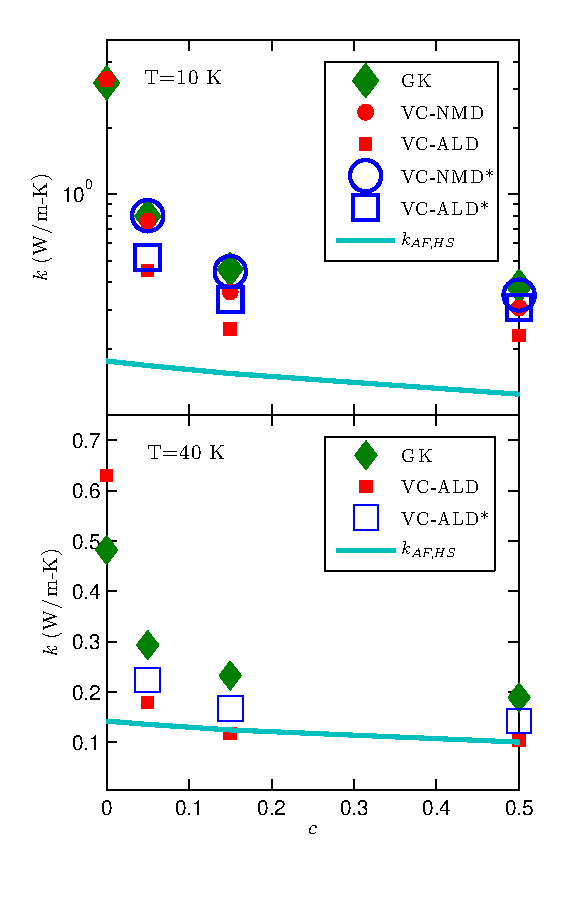
\includegraphics[scale=1.0]
{/home/jason/disorder/lj/alloy/lj_cond_compare.eps}
\vspace*{-5mm}
\end{center}
\caption{\label{F:cond_lj} (a) thermal conductivity predictions for 
LJ argon alloys at T=10K using the VC-NMD, VC-ALD, and GK methods. (b) 
thermal conductivity predictions at T=40K.}
\end{figure}
%--------------------------------------------------------------------------

%--------------------------------------------------------------------------
\begin{figure}
\begin{center}
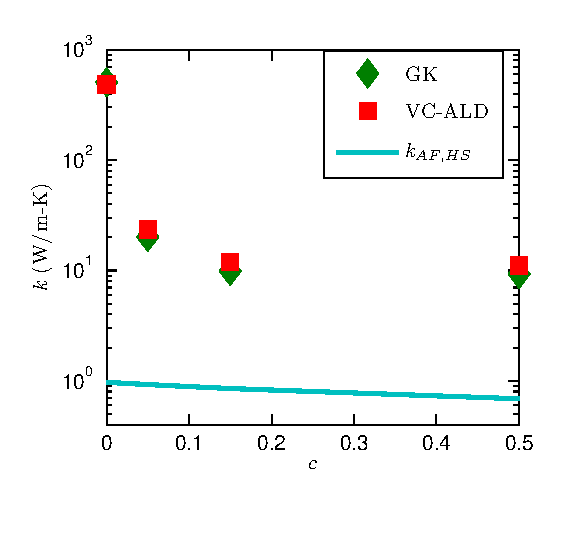
\includegraphics[scale=1.0]
{/home/jason/disorder/si/alloy/m_si_cond_compare.eps}
\vspace*{-5mm}
\end{center}
\caption{\label{F:cond_si} }
\end{figure}
%--------------------------------------------------------------------------

% %--------------------------------------------------------------------------
% \begin{figure}
% \begin{center}
% \includegraphics[scale=1.0]
% {/home/jason/disorder/pbte/m_pbte_cond_compare.eps}
% \vspace*{-5mm}
% \end{center}
% \caption{\label{F:conductivity_lj} }
% \end{figure}
% %--------------------------------------------------------------------------

%--------------------------------------------------------------------------
\section{\label{S:Discussion}Discussion}
%--------------------------------------------------------------------------

The LJ argon and SW silicon alloys studied in this work 
have different ranges of phonon frequencies, 
lifetimes, group velocities and total thermal conductivity. 
For bulk silicon(cite), the thermal conductivity 
is dominated by low-frequency modes(cite), which is also true for 
bulk and alloyed SW silicon (Fig. \ref{F:Dph_si}).(cite) For SW silicon, 
VC-ALD predicts thermal conductivities in reasonably 
good agreement with the 
explicitly disordered GK method (Fig. \ref{F:cond_si}).  
For LJ argon, VC-ALD underpredicts 
the high-frequency phonon lifetimes and thermal diffusivities 
(Fig. \ref{F:Dph_lj}), 
leading to an underprediction of 
thermal conductivity when compared to VC-NMD and GK 
(Section \ref{S:Thermal Conductivity}). 

The results for SW silicon and LJ argon alloys suggest that 
the thermal modeling of ordered and 
disordered lattices can be separated into two broad groups: 
low- and high-frequency dominated materials.(cite) Materials dominated 
by low-frequency modes tend to have high thermal conductivities, 
which is due to their large group velocities and long lifetimes.
(cite) These low-frequency modes  
follow closely the scalings predicted by the perturbative VC-ALD 
models, which are valid at low-frequencies. 

LJ argon is a material 
dominated by high-frequency modes, even for the bulk 
(Fig. \ref{F:Dph_lj}). 
This high-frequency range is where the perturbative VC-ALD models, 
and also where the higher-order 
terms in the Tamura theory are predicted to be non-negligible 
(Section \ref{S:From VC-ALD}). 
While the 
high-order terms in the Tamura theory are also predicted to be 
non-negligible for SW silicon, this does not affect the thermal 
conductivty predictions signifcantly. Even if there was a discrepancy 
at high-frequency these modes 
are unimportant to thermal transport in SW silicon. This is also 
true for the thermal conductivity spectrum of SiGe alloys 
from first-princples predictions\cite{garg_role_2011} and experimental 
measurements.\cite{abeles_thermal_1962,cahill_thermal_2004,
cahill_thermal_2005,cheaito_experimental_2012} 
and first-principles predictions\cite{garg_role_2011,lindsay_thermal_2012} 
this is also true for SiGe alloys and isotopic GaN.
\cite{} 
For example, the thermal conductivity of SiGe alloys
exceeds the high-scatter limit by more than
an order of magnitude at room temperature for all com-
positions.

Resolution 
of the breakdown of the perturbative VC-ALD models for LJ argon 
is achieved by considering the thermal diffusivity of vibrational 
modes in the AF theory. 
A simple correction to the VC approximation can be made by considering 
a high-scatter limit for the mode specific thermal 
diffusivity (Section \ref{S:Diffusivities}). 
This high-scatter limit is physically interpreted as vibrational modes 
propagating at the sound speed a distance of the lattice constant. 
However, the concept of a vibrational mean free path 
in a disordered system is only valid at low-frequencies.
\cite{feldman_numerical_1999,xu_energy_2009} For 
disordered vibrations, the lifetime and thermal diffusivity are the 
fundamental quantities. The VC approximation underpredicts 
the mode thermal 
diffusivity due to disorder because the group velocities $v_g\kv$ can 
approach zero (Section ), though this is a small effect compared to 
the underprediction of the lifetimes by VC-ALD. 

For LJ argon, it is possible that the VC group velocities are an 
over-prediction for modes in a given interval of frequency, 
an effect which is compensated for 
by a small under-prediction of the lifetimes in the same interval of 
frequency when compared to Gamma-NMD (Fig. \ref{F:VC Gamma life}). 
The VC-NMD predicted 
mode lifetimes and thermal diffusivity adjusted VC-NMD$^*$, 
predict thermal conducitivities in good agreement with 
the MD-based GK method. 
Based on the thermal conductivity predictions for VC-NMD$^*$ and 
the well-defined peaks in the structure factors 
(Fig. \ref{F:SF}), the reduction of group velocities in 
disordered lattices 
due to zone folding seems to be an underprediction of the group 
velocity of moderate to high frequency modes.\cite{duda_reducing_2011}  

% As observed by Kittel, if the sound
% velocity is used instead of U; and the interatomic spacing
% is used instead of the mean free path l;, then tc( T) is qual-
% itatively and semiquantitatively
% fit at temperatures above
% the plateau region.
% In fact, Slack showed that the same model 
% is useful for crystalline insulators with strong scattering.(waiting for 
% ILL).\cite{henry_ehrenreich_thermal_1979}

% The theory by Tamura is able to treat disorder scattering in an arbitrary 
% crystal with dispersion. The theory, however, fails to predict the 
% lifetimes of high-frequency modes, which are critical to the total 
% thermal conductivity in LJ argon (see Fig. and ). To match the predicted 
% phonon lifetime at high fequency for $c=0.05$ 
% ($\tau\kv \propto const.$, Fig. ), 
% the Tamura theory (to order 2, $g_2(b)$) requires a DOS which scales as 
% $D(\omega\kv) \propto const.$. Clearly from Fig. , this is not the case 
% with either the VC or Gamma modes. To match the predicted 
% phonon lifetime at high fequency for $c=0.5$ 
% ($\tau\kv \propto 1/\omega\kv$, Fig. , also true for all $c$ in SW silicon), 
% The higher-order terms in the Tamura theory are demonstrated to be large 
% in Fig., but it is unclear if and how they are responsible for the 
% underpredictions of the VC-ALD method for LJ argon. 

% While Broido found that omission of optical scattering overpredicts 
% the thermal 
% conductivity of bulk Si by a factor of 2-3, 
% optical modes contribute less than $5\%$ 
% to thermal conductivity itself. Similarly, the diffusivity adjusted 
% thermal 
% cobductivities of SW Si are increased by less then about $1\%$, 
% demonstrating the 
% the high frequency and optical modes are also unimportant to thermal 
% transport 
% in Si alloys. 

% For the perfect system, phonon modes with nearly zero group velocity 
% (optical modes and acoustic modes at the BZ boundaries) have essentially 
% zero thermal diffusivity and contribute nearly 
% nothing to the thermal transport, while the modes themselves 
% are important to the 
% scattering of other phonons.(cite) In the disordered lattices under the 
% AF theory, modes important to thermal transport have a finite thermal 
% diffusivity, as opposed to  the minimum $D_{th} \approx 0 $ for phonons 
% in a perfect lattice. This finite thermal diffusivity limit is the cause 
% for the large (LJ argon Fig. ) and small (SW silicon Fig. ) 
% descrepcny between the thermal conductivity prdictions of VC-ALD and 
% VC-NMD versus 

% High thermal conductivity materials tend to have a conductivity spectrum 
% which is peaked in the low frequency range.(cite) 
% It is in this range where the mode 
% lifetimes follow closely the scalings with frequency which can be 
% predicted by the perturbative models for intrinsic and disorder 
% scattering as 
% (Section Eq. ).

% In contrast, 
% in LJ argon the high frequency phonon mode properties are critical 
% to the thermal transport.(cite)  
% While the low frequency phonon properties predicted by VC-NMD and 
% VC-ALD agree, it is the failure of the perturbative models at 
% high frequency which causes VC-ALD to underpredict. The failure 
% to account for harmonic disordered scattering due to the AF theory 
% is responsible for causing both VC-NMD and VC-ALD to underpredict 
% versus GK, which affects the high frequency modes significantly. 
% LJ argon, with lower 
% frequencies, lifetimes, and group velocities compared to 
% ``stiff'' SW silicon, 
% is considered a ``soft'' system. 

% For SW silicon, the low frequency modes dominate thermal transport 
% even in the heavily disordered alloy.(cite new Hopkins) 
% It is thus unsurprising that predictions for 
% SW silicon using VC-ALD agree well with VC-NMD and GK. This is also a 
% plausible explanation for the success of predictions using 
% VC-ALD and ab initio calculations compared to experiment for 
% ``stiff'' systems (i.e. Si-Ge).(cite)

%--------------------------------------------------------------------------
\section{\label{S:Summary}Summary}
%--------------------------------------------------------------------------

The concept of simple alloying is at the forefront of the effort 
to control or minimize the thermal conductivity of semiconducting and 
thermoeletric materials (cite SiGe nanoporous, PbTe) 
Results in this work suggest that the lower limit for the vibrational 
mode thermal diffusivity in alloys with thermal conductivities near the 
high-scatter limit is $(1/3)v_sa$. 
Such materials include the thermoelectric PbTe,
particularly at the high operating termperatures of thermoelectric 
energy generation.(cite) PbTe has a thermal conductivity in the 
mid-range of frequencies, placing it between SW silicon and 
LJ argon. The optical phonons in PbTe/PbSe alloys have been 
predicted to have group velocities 
as large as the acoustic branches, 
making PbTe/PbSe distinctly unique compared 
to SW silicon or LJ argon alloys.
\cite{tian_phonon_2012} 
It is not clear what role the high-scatter limit of the mode-specific 
thermal diffusivity has in predictions for PbTe/PbSe alloys. 

The results in this work support the idea of a minimum thermal diffusivity 
for the vibrations in disordered lattices.(cite) 
Although this minimum thermal 
diffusivity is usually interpreted as a minimum mean free path, we find 
that concept is not necessary for interpreting the results. The VC 
approximation provides a computationally cheap framework, which is 
essential for expensive but experimentally accurate \emph{ab initio} 
methods for predicting thermal conductivity.(cite) 
The high-scatter limit 
of thermal diffusivity is more useful for examing the thermal transport 
in alloys under the framework of the VC approximation. The 
fundamental quantity is the mode lifetimes and the group velocity 
is an approximation, and expressed together as thermal diffusivity 
they can be interpreted in the presence of disorder.

\begin{acknowledgements}
This work was supported in part by a grant of computer time from the DOD 
High Performance Computing Modernization Program at the US Army Engineer 
Research and Development Center. 
We thank Jivtesh Garg, Zhiting Tian, Davide Donadio, 
Asad Hasan and Craig Maloney for helpful discussions.
\end{acknowledgements}

%--------------------------------------------------------------------------
\appendix
%--------------------------------------------------------------------------

%--------------------------------------------------------------------------
\section{\label{A:Computational Cost}
Computational Cost}
%--------------------------------------------------------------------------

The key to incorporating the effects of disorder explicitly are the use 
of a large disordered supercells (Section \ref{S:Calculation}). 
However, the methods used 
in this work scale differently with the size of the supercell considered. 
The calculations in this work are trivially parallelizable\cite{} 
except the 
MD simulations\cite{plimpton_fast_1995} and the eigenvalue solution of the 
Dynamical matrix.\cite{gale_general_2003} Efficient MD 
codes scale linearly with the number of atoms in the system $N_a$, making 
the GK method an efficient method for predicting thermal conductivity. 
However, the computational cost of using large supercells for MD simulation, 
particularly because of the large number of time steps required 
(on the order of $10^5 - 10^7$ depending on the 
system, time step used, etc (cite)), prohibit its use with typical 
\emph{ab initio} methods such as 
plane-wave Density Functional Theory.(cite) 

Both VC-NMD and VC-ALD require the eigenvalue solution 
of a Dynamical matrix of size $(3n,3n)$ for each irreducible wavevector 
of the system size considered, 
which is negligible compared to the other 
caculations required for both of these methods.(cite) 
The Gamma-NMD (Section \ref{S:VC Gamma life}) and 
AF theory (Section \ref{S:Diffusivities}) 
require the eigenvalue solution of a large Dynamical matrix $(3N_a,3N_a)$, 
the solution of which scales as $(3N_a)^3$. 
The AF theory is limited 
to small supercells using ab initio calculations, making it difficult 
to asses finite-size effects.(cite)  

Using the VC-ALD method, the symmetries of the system can be 
used to drastically reduce the required computations, permitting its 
use with ab initio methods.
\cite{esfarjani_method_2008,turney_predicting_2009,
esfarjani_heat_2011,chaput_phonon-phonon_2011} 
For VC-ALD, the calculation of the intrinsic phonon 
lifetimes $\tau_{p-p}\kv$ scales as $n^4$,\cite{turney_predicting_2009}  
making calcualtions for large unit cells challenging.(cite) 
Compared to 
the calculation of the intrinsic phonon lifetimes, calculation 
of the defect lifetimes $\tau_d\kv$ (Eq. ) is negligible.

% Consider the following computational times for the methods used in 
% this work for LJ argon and $N_0 = 12$. All calculations were performed 
% on the same computing cluster and include the effect of using 
% multiple processors (for example the VC-ALD calculations were run using 
% 12 cpu for 4.1 hours):
% 
% AF = eigenvalue solution + thermal diffusivity calculation = 4.2 hours
% 
% VC-ALD time = 49.2 hours?
% 
% VC-NMD time = 102 hours for MD + 780 hours for NMD + negligible time 
% to generate phonon frequencies and eigenvectors
% 
% LJ VC-Gamma = MD simulation + NMD + eigenvalue solution =  
% 102 hours + 780 hours + 3.8 hours = 
% 
% Parallel eigenvalue solvers exist for most ab initio packages, required 
% to solve for the eigenvalues of the Hamiltonian matrix.(cite) Incorporating 
% parallel eigenvalue solvers into existing 
% Sparse eigenvalue solutions may be implemented for systems which are 
% large enough and have short-range interactions.(cite)

% \begin{center}
% \begin{table}
% \caption{\label{T:cond_table}Thermal conductivity values in W/m-K predicted using the $\Phi$, 
% $\Phi'$, and Green-Kubo methods.  The predictions for $\Phi$ and Green-Kubo for the LJ system 
% are in good agreement with those from other atomistic simulation methods\cite{turney2009a} while 
% those from $\Phi'$ differ and show no consistent behavior. The uncertainties in the predicted thermal 
% conductivities for $\Phi$ and $\Phi'$ come predominantly from the finite simulation-size scaling 
% procedure (see Ref. \cite{turney2009a,He2011a}), where the phonon properties and thermal conductivity 
% are predicted for increasing system sizes ($N_1=N_2=N_3$) to extrapolate a bulk thermal conductivity. 
% For SW silicon and the CNT, the extrapolation procedure is not performed. }
% \begin{ruledtabular}
% \begin{tabular}{llllll}
%      &                             &         &      &   \\
% $T$ (K)&Green-Kubo \ &$\Phi$ &$\Phi'$\\
% \hline
% LJ (bulk)\\
% 5&8.0 $\pm$ 0.30 &7.9 $\pm$ 0.42 &5.8 $\pm$ 0.31 \\
% 20&1.3 $\pm$ 0.15 &1.2 $\pm$ 0.07 &1.0 $\pm$ 0.10 \\
% 40&0.45 $\pm$ 0.07 &0.47 $\pm$ 0.03 &0.49 $\pm$ 0.05 \\
% \hline
% SW ($N_1=N_2=N_3=6$) \\
% 300& &322 $\pm$ 16 &396 $\pm$ 38 \\
% \hline
% CNT ($N_1=N_2=1, N_3=50$) \\
% 300& &428 $\pm$ 21 &398 $\pm$ 40 \\
% \end{tabular}
% \end{ruledtabular}
% \end{table}
% \end{center}

%MD: Loop time of 2021.86 on 12 procs for 1000000 steps with 6912 atoms
%matlab NMD: /home/jason/lammps/LJ/alloy/10K/0.5/12x/NMD/1
%35261.719809 for one NMD_1_1

%--------------------------------------------------------------------------
\section{\label{A:NMD XCORR}
NMD using Non-Exact Normal Modes}
%--------------------------------------------------------------------------

The NMD method reuquires the atomic positions and velocities  
from an MD simulation.(cite) 
The MD simulations are performed using the package LAMMPS.
\cite{plimpton_fast_1995} The lengths of the MD simulations were longer 
than 10 times the longest phonon lifetime in the system. These can 
be estimated a priori from the VC-ALD predicted phonon lifetimes. For LJ 
argon and SW silicon, the simulations were run using time steps of 
$dt=0.002$ LJ units and $dt = 0.0005 fs$ for $2^20$ and 
$2^22$ time steps and the atomic trajectories were sampled 
every $2^8$ and $2^4$ time steps, respectively. 
Ensemble averaging was performed using 10 independent initial 
randomized velocity distributions. 

For a normal mode of the lattice supercell 
used for the MD simulations, 
the autocorrelation of the total and kinetic     
normal mode energy are damped exponentials 
with a decay time $\tau\kv$, the kinetic energy autocorrelation with a 
cosinusodial oscillation frequency 
$2\omega\kv$.(cite joe) 
When using the VC normal modes to map the MD simulation 
trajectories for the explicitly disordered lattice supercells, 
the mode total and kinetic energy autocorrelation fucntions 
do not always follow simple functional forms. 
This can be illustrated by using spectral-NMD 
in the frequency domain, where artifacts such as 
multiple peaks in an isolated mode's 
energy spectrum ($\Phi$) can be observed (see Fig ).(cite)  
In the case 
of multiple peaks, the choice of which peak to fit to predict the phonon 
properties can be ambiguous.  However, 
a lifetime can be predicted unambiguously using Eq. even with 
these multiple-peak artifacts, particularly because the autocorrelations 
are damped exponentially. This results is to be expected 
given that the atomic trajectories contain 
information about the lattice energy, which from general statistical 
physics principles will have exponential relaxation behavior in an 
equillibrium ensemble.
\cite{srivastava_physics_1990,landau_statistical_1980,
rajabpour_thermal_2010}

These artifacts are not surprising given two considerations: 
1) the MD simulations 
contain explicit disorder which incluences the atomic trajectories 2)
the VC normal modes are not the exact normal modes and of the 
explicitly disordered system. 
Descrepencies have been observed previously when the exact normal modes 
of the system are not used.(cite SED) However, the lifetimes predicted 
using VC-NMD are in fairly good agreement with those calculated using 
Gamma-NMD (Fig. \ref{F:VC Gamma life}). 
Several studies have found good agreement for 
predictions of lifetimes and thermal conductivity 
using non-exact eigenvector mappings
\cite{koker_thermal_2009,thomas_predicting_2010} 
in a wide-range of materials and 
phonon scattering conditions.
\cite{
koker_thermal_2009,thomas_predicting_2010,shiomi_thermal_2011,
ong_reduction_2011,qiu_molecular_2012} 
However, it is crucial 
that results using non-exact mappings are compared to as many 
alternative methods as possible. In this work, VC-NMD is 
compared to the other methods Gamma-NMD 
(Section \ref{S:VC Gamma life}), 
GK (Section \ref{S:Thermal Conductivty}), 
and VC-ALD (Section \ref{S:Diffusivities}).
It is important to remember that the VC normal modes 
are exact in the limit $c->0$. 
Use of the VC 
modes at large $c$ pushes the limits of the approximation, but  
is useful for predicting an effective group velocity 
(Section \ref{S:Dispersion}).

%--------------------------------------------------------------------------
\begin{figure}
\begin{center}
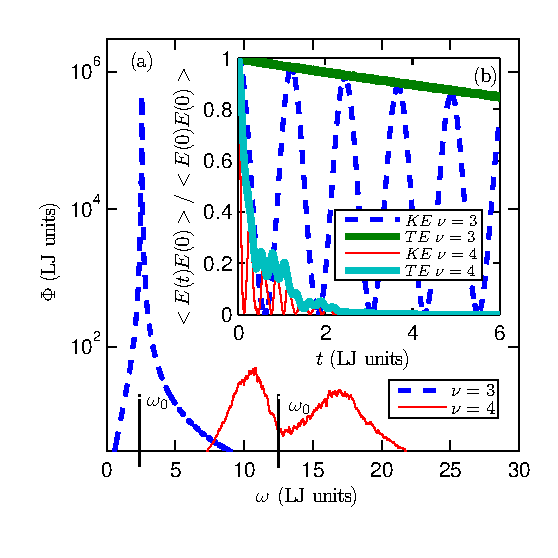
\includegraphics[scale=0.75]
{/home/jason/disorder/lj/alloy/m_lj_nmd_xcorr_compare.eps}
\vspace*{-5mm}
\end{center}
\caption{\label{F:NMD XCORR} The spectral energy density $\Phi$ of 
two modes (polarizations $\nu=3,4$ at wavector [0.2 0 0]) calculated 
using VC-NMD for a mass disordered LJ FCC supercell 
($N_0=8$ and $c=0.5$). 
The VC dispersion-predicted peaks are labeled 
by $\omega_0$. Inset: the same mode's energy 
(kinetic (KE) and total (TE)) autocorrleation functions.  
Note the additional 
harmonic effects in the KE and TE autoccorelation functions 
for $\nu=4$ which are due to the double peaks in $\Phi$. 
A mode lifetime can 
be extracted unambiguously using the integral of the TE autocorrelation 
function (Section \ref{S:VC Gamma life}).}
\end{figure}
%--------------------------------------------------------------------------


%--------------------------------------------------------------------------
\section{\label{A:SF}Calculation of the Gamma Mode Structure Factors}
%--------------------------------------------------------------------------

To calculate 
$S^{L,T}\kw$ for a finite-size system, the 
delta function in Eq. \eqref{EQ:M:SLT} is broadened using a Lorentzian 
function with a full-width at half maximum 
$\Gamma_{FMHW} = \delta_{\omega,avg}$, 
where 
$\delta_{\omega,avg}$ is the average frequency spacing. 
Allen et al\cite{allen_diffusons_1999} 
demonstrated using a model of 
a-Si that the structure factor 
for large wavevector broadens so that the 
linewidth $\Gamma_{SF} > \omega$.
\cite{taraskin_determination_1999}
For the systems sizes studied, $\Gamma_{SF}$ 
scale with the brodening factor 
$\Gamma_{FMHW}$ for all peaks 
except those at high frequencies. 

For the range of broadening factors 
considered ($\Gamma_{FMHW} = \delta_{\omega,avg}$ to $50\delta_{\omega,avg}$) 
the linedwidths extracted for all $c$ 
generally satisfy $\Gamma_{SF} > \omega$. 
For all broadening factors, the linewidths 
(inverse lifetimes, $\tau_{SF} = 1/2\Gamma_{SF}$) 
at high frequency are in better 
agreement with the lifetimes predicted 
by VC-NMD rather than VC-ALD,
where generally $\tau > 2\pi/\omega$ 
(IR limit, Fig. \ref{F:VC Gamma life}).
\cite{taraskin_determination_1999} This gives more  
justification for the use of the VC predicted group velcoities for 
both VC-NMD and VC-ALD, even for large wavevector and $c$. 

In general, the polarization of the eigenvectors $e\kvba$ will not 
be purely transverse or logitudinal along the reciprocal directions. 
Even for the simple LJ argon system, this can make it difficult to 
uniquely identify then different polarizations with the various 
peaks in the structure factors. For SW silicon, similar good agreement 
can be seen along the high symmetry directions for the acoustic branches, 
while the optical modes 
and more complicated polarizations are too difficult to identify in 
an automated way. 
In general, the acoustic branches can be identified, provided they are 
well separated in frequency from any optical branches.
\cite{feldman_numerical_1999,thomas_predicting_2010} 

%--------------------------------------------------------------------------
\section{\label{A:Finite Simulation}
Finite Simulation-Size Scaling for Thermal 
Conductivity}
%--------------------------------------------------------------------------
To predict a bulk thermal conductivity, extrapolation is used by the 
following finite size scaling $ 1 / k \propto 1/N_0$. For VC-NMD and 
VC-ALD, the validity of the finite-size scaling 
requires the low frequency modes in the finite system to be dominated by 
intrinsic scattering ($\tau\kv \propto \omega\kv^{-2}$) and  
follow the Debye approximation 
with respect to $v_{g,\mathbf{n}}$ and DOS $D(\omega\kv)$.
\cite{shiomi_thermal_2011,esfarjani_heat_2011} For LJ 
argon, this requirement is satisfied for modest system sizes 
(for $N_0 = 6$ to $12$) so that both VC-NMD and VC-ALD predictions 
can be extrapolated to a bulk value. 
For SW silicon, the thermal conductivity is dominated by low-frequency 
modes (Fig. \ref{F:Dph_si}). Becasue of this, large system sizes 
(up to $N_0 = 42$) are needed to satsify the 
extrpaolation requirements and only VC-ALD can be used.(cite) This 
demonstrates the computational efficieny of the VC-ALD method which is 
necessary when computationally expensive 
ab initio methods are used (Section ).
\cite{garg_role_2011,tian_phonon_2012,
lindsay_thermal_2012,esfarjani_heat_2011}

System sizes of up to $N_0=38$ are required to predict converged 
thermal conductivity of SW silicon alloys. 
For Si modeled using the Tersoff potential, 
system sizes of up to 64000 atoms are required to observe 
converged values of thermal conductivity using the GK method.
\cite{he_lattice_2012} We find that similar system sizes are 
also required for 

For the GK method, smaller system sizes $N_0 \le 12$ are used for the 
finite size extrapolation for LJ argon and SW silicon . 
The validity of this result can be explained in terms of a 
combination of effects which are specific to the MD simulations.
\cite{esfarjani_heat_2011} In fact, for $c=0$ the GK results are 
independent of system size for $N_0 = 4$ to $N_0 = 12$ for LJ argon.

\clearpage
\bibliographystyle{apsrev}
%\bibliography{/home/jason/sed/jop/asme_prb_paper/prb/references}
\bibliography{/home/jason/Dropbox/ntpl-paper/ntpl-021313}
\end{document}
